\documentclass[aps,prd,twocolumn,10pt,superscriptaddress,nofootinbib,longbibliography,floatfix]{revtex4-2}

\usepackage{amsmath,amssymb,amsfonts}
\usepackage{bm}
\usepackage{graphicx}
\usepackage{booktabs}
\usepackage{xcolor}
\usepackage{hyperref}
\graphicspath{{figures/}}
\hypersetup{colorlinks=true,linkcolor=blue,citecolor=blue,urlcolor=blue}

\newcommand{\dd}{\mathrm{d}}
\newcommand{\Mpl}{M_\mathrm{Pl}}
\newcommand{\Ham}{\mathcal{H}}
\newcommand{\Mom}{\mathcal{M}}
\newcommand{\Pone}{Paper~I}
\newcommand{\Ptwo}{Paper~II}
\newcommand{\pending}[1]{\textcolor{red}{[Pending: #1]}}

\begin{document}
\raggedbottom

\title{Stochastic inflation in general relativity, on a lattice and in one patch:\\ A reproduction of two papers (working note)}

\author{Track E of the numerical-relativity particle-in-cell cosmology program}

\date{Working note, state of 24 November 2026}

\begin{abstract}
Stochastic inflation adds the quantum noise of modes that cross a coarse-graining scale to the evolution of long-wavelength fields. Launay, Rigopoulos and Shellard wrote this noise as sources for every Einstein equation, integrated a one-patch Langevin system for the lapse and the local number of e-folds, and evolved the sources on a numerical-relativity lattice for a slow-roll and an ultra-slow-roll potential. We reproduce both papers in their own set-up: the lattice part with an independent numerical-relativity code, the one-patch part with a reference integrator. Computer algebra confirms that the sources are independent of the gauge and leave the constraints unsourced at linear order. On the lattice, the background, the spectra of the curvature perturbation and of the extrinsic curvature, the freezing of super-Hubble modes, the order of the constraint violation and the convergence with resolution agree with the published runs and with linear theory. The spread of the fields over the lattice is three to four times narrower in our runs than in the published figures, in both scenarios, while the published spectra agree with ours, and the spectra fix the spread. The published bound on the stochastic backreaction holds at large scales and fails at the shortest scales of ultra-slow roll, as the published figure itself shows. The one-patch figures follow only from a background integrated with a coarse Euler step, which carries the field off a plateau where the converged background stops, and from the It\^o reading of the printed equation. The It\^o correction carries the fifth power of the lapse, and the ultra-slow-roll noise amplitude is smaller than printed. A second agent that produced none of the runs recomputed, from the raw outputs and with its own code, the background, the spectra, the constraint records, the amplitude factor, the plateau stop, the It\^o reading, the It\^o term and the ultra-slow-roll amplitude, and confirmed them; it did not recompute the extrinsic-curvature spectra or the gauge families. On the finest lattice the spectra stop converging at the longest scales, at a floor that does not depend on the spacing or the step and has the size of the second-order terms of the field. In slow roll the Hamiltonian violation of single cells reaches the published level at the last crossings and then decays. Judged against nine criteria fixed before the runs, the ultra-slow-roll lattice meets every criterion but one: at one record time the momentum constraint misses the second-order scaling with the noise amplitude that the criterion demands. Runs at three amplitudes show, after the data, that the miss comes from the estimator of the noise level fixed in advance, and the failure stays on record.
\end{abstract}

\maketitle

\section{Introduction}\label{sec:intro}

Primordial black holes form where the comoving curvature perturbation of inflation is large enough for a region to collapse after it re-enters the Hubble radius, so their abundance depends on the far tail of its distribution. Stochastic inflation describes how that tail grows. Modes that cross a coarse-graining scale, a fixed fraction of the Hubble radius, feed a classical noise into the long-wavelength fields \cite{Starobinsky:1986}. The usual form evolves every coarse-grained patch as a homogeneous universe, which drops gradients and the anisotropic part of the expansion.

Launay, Rigopoulos and Shellard removed that restriction. In the first paper (\Pone{} \cite{Launay:2024sigr}) they wrote the noise as sources for every equation of general relativity in its 3+1 form, built from the comoving curvature perturbation and the time derivatives of the window, and tested the result on a one-patch Langevin system for the lapse and the local number of e-folds in the uniform-field gauge. In the second (\Ptwo{} \cite{Launay:2025sinr}) they derived the sources without fixing a gauge, cast them in the BSSN form of numerical relativity, and evolved them on a lattice for a slow-roll (SR) and an ultra-slow-roll (USR) potential, starting from the initial data of Ref.~\cite{Launay:2025bd}.

A reproduction tests what the two papers print: equations, set-up, figures and quantitative statements. Neither the authors' code nor their random numbers are public, so the comparison is statistical, against the linear (Mukhanov--Sasaki) solution of each realization, and against the numbers the papers print. Values read off the published figures enter only as single comparison values, with the figure named, in the ledger at the end of the note. Figure~\ref{fig:pipeline} shows the two reproductions side by side. The work was carried out by large-language-model agents under human direction, who wrote the specification, ran the simulations, checked the equations and wrote this note. A further agent, which had produced none of the runs and was given the raw outputs and the list of claims but not our conclusions, recomputed the claims with its own readers, references and integrators. Its verdict on each statement stands in Appendix~\ref{app:verdicts} and on each number in the ledger.

This note reports four results:
(i) the equations of both papers hold under computer algebra; the misprints we found do not enter a code (Sec.~\ref{sec:equations});
(ii) on the lattice, every observable that linear theory fixes is reproduced, the one-point spread of the fields is not, and the constraint levels and the bound on the backreaction follow from it and from the published figures (Sec.~\ref{sec:lattice});
(iii) in one patch, the published figures require a background integrated with a coarse Euler step and the It\^o reading of the printed equation, whose It\^o term and ultra-slow-roll amplitude differ from the printed forms (Sec.~\ref{sec:onepatch});
(iv) judged against criteria fixed before the runs, the ultra-slow-roll lattice meets every criterion but one, the second-order scaling of the momentum constraint at one record time (Sec.~\ref{sec:criteria}).
Section~\ref{sec:discussion} sorts the findings into reproduced, reproduced in part, not reproduced and open.

\begin{figure*}
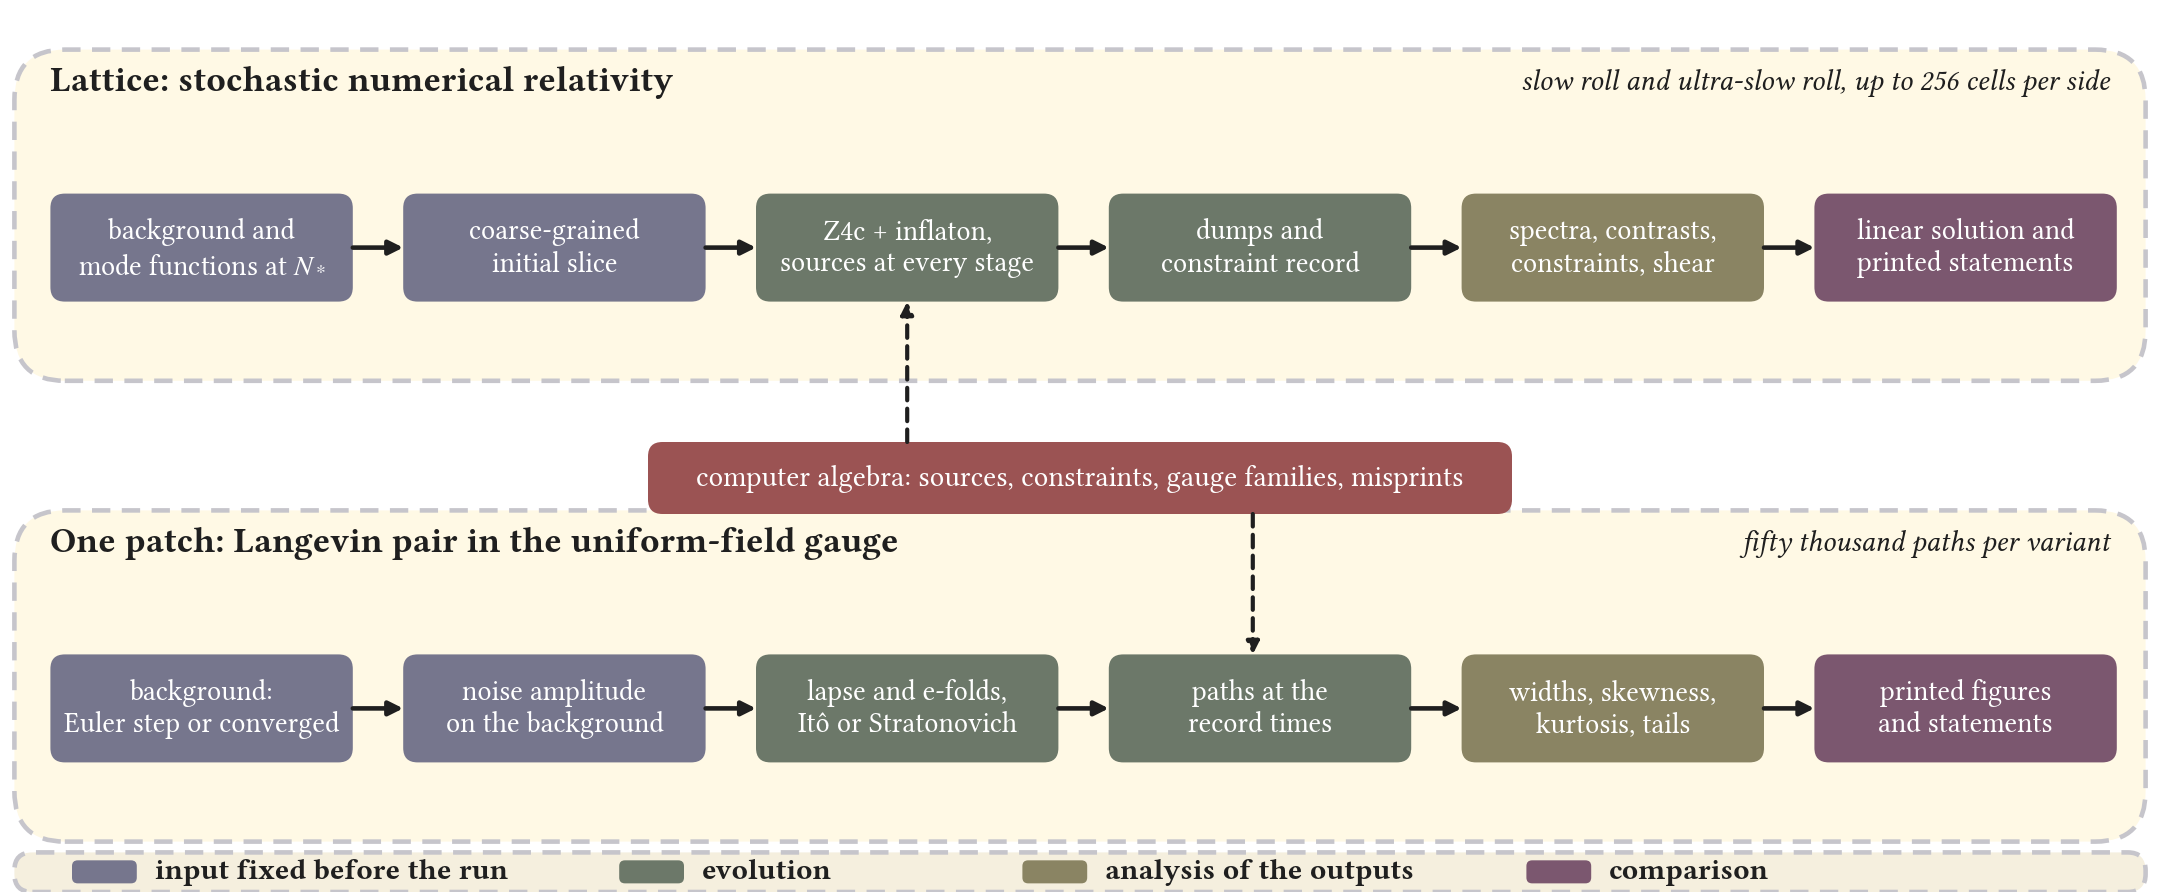
\includegraphics[width=\textwidth]{fig_pipeline}
\caption{The two reproductions. Top: the lattice of \Ptwo{}, from the initial data at the start of the run to the comparison with linear theory. Bottom: the one-patch system of \Pone{}. Middle: the computer-algebra check of the equations, which both lanes use. Colors mark inputs, evolution, analysis and comparison.}
\label{fig:pipeline}
\end{figure*}

\section{Stochastic sources in general relativity}\label{sec:equations}

A coarse-graining window splits every field into a long-wavelength part, which the simulation evolves, and a short-wavelength part, which linear theory describes. Both papers use a smooth window in Fourier space,
\begin{equation}
W_k(t) = \tfrac{1}{2}\left\{1 + \tanh\left[s \ln\left(k_\sigma/k\right)\right]\right\}, \qquad k_\sigma = \sigma a H,
\label{eq:window}
\end{equation}
where $a$ is the scale factor, $H$ the Hubble rate, $\sigma$ the window scale in units of the Hubble scale and $s$ the steepness. As $aH$ grows, each mode slides from the short part into the long part, and the long part receives a kick.

The kick follows from linear theory. The mode function $\mathcal{R}_k$ of the comoving curvature perturbation obeys the Mukhanov--Sasaki equation \cite{Sasaki:1986,Mukhanov:1988}
\begin{equation}
\ddot{\mathcal{R}}_k + (3-\epsilon_2) H \dot{\mathcal{R}}_k + \frac{k^2}{a^2} \mathcal{R}_k = 0,
\label{eq:ms}
\end{equation}
with $\epsilon_1 = -\dd\ln H/\dd\mathcal{N}$, $\epsilon_2 = -\dd\ln\epsilon_1/\dd\mathcal{N}$ (the sign of both papers, so $\epsilon_2 = 6$ in USR) and $\mathcal{N}$ the number of e-folds. Applying the same operator to the windowed mode $W_k \mathcal{R}_k$ and using the Mukhanov--Sasaki equation leaves only the terms with derivatives of the window,
\begin{equation}
S_{\mathcal{R},k} = \mathcal{R}_k \ddot W_k + \left[2\dot{\mathcal{R}}_k + (3-\epsilon_2) H \mathcal{R}_k\right] \dot W_k .
\label{eq:sr}
\end{equation}
The coarse-grained curvature perturbation therefore obeys the Mukhanov--Sasaki equation with the source $S_\mathcal{R}$, the sum of $S_{\mathcal{R},k}$ over the modes, each weighted by a complex Gaussian random number drawn once. The papers carry this source into the field momentum $\Pi$, the trace $K$ of the extrinsic curvature and its trace-free part $\tilde A_{ij}$:
\begin{equation}
\begin{aligned}
S_\Pi &= \sqrt{2\epsilon_1}\,\Mpl S_\mathcal{R}, \qquad S_K = -\epsilon_1 S_\mathcal{R}, \\
S_{\tilde A_{ij}} &= \epsilon_1\left(\frac{\delta_{ij}}{3} - \frac{k_i k_j}{k^2}\right) S_\mathcal{R},
\end{aligned}
\label{eq:sources}
\end{equation}
with no source in the metric, in the other evolved variables or in the constraints. We call these the stochastic sources.

We linearized the nonlinear 3+1 equations about a flat Friedmann background for one plane wave and substituted five gauge families of \Pone{}, each with arbitrary gauge functions. In every family the residuals equal the stochastic sources, and the linearized Hamiltonian and momentum constraints receive no source. Flipping the sign of any one source makes the time derivative of a constraint nonzero at first order. This property turns the constraints into a test of the noise on the lattice: a correct source keeps the Hamiltonian violation at second order in the noise, a wrong sign raises it to first order.

The coefficients $\epsilon_1$, $\epsilon_2$, $H$ and $a$ of the sources belong to a background. \Ptwo{} offers three choices: the Friedmann background (level 0 of the backreaction), the box means of the lattice (level 1), and the local fields in each cell (level 2). Level 2 is its production setting.

The checks also found seventeen misprints in the two papers (Table~\ref{tab:errata} in Appendix~\ref{app:errata}): a misplaced prefactor in the linear momentum constraint, a delta that should be the metric in the trace-free equation, missing factors in the Friedmann line of the usual stochastic equations, a factor $4\pi$ in a system written with $\Mpl$, and the two findings about the one-patch system of Sec.~\ref{sec:onepatch}. None of them enters the lattice code.

\section{The lattice reproduction}\label{sec:lattice}

\subsection{Two scenarios and our set-up}\label{sec:setup}

In the SR scenario the inflaton rolls down a quadratic potential. Every mode enters the window, rises to a nearly scale-invariant spectrum and freezes once it is far outside the Hubble radius. In the USR scenario the potential has an inflection point: the field decelerates on a nearly flat stretch, $\epsilon_1$ falls by many decades, and the curvature perturbation of modes already outside the Hubble radius grows until the field leaves the plateau. The spectrum then rises steeply toward small scales.

\Ptwo{} evolves the BSSN equations \cite{Shibata:1995,Baumgarte:1998} with geodesic slicing in a periodic box one window wavelength across at the start, with a noise cut-off at a quarter of the Nyquist wave number, $\sigma = 1$, $s = 5$, sixth-order finite differences, the classical fourth-order Runge--Kutta method and no dissipation. We use AthenaK \cite{Stone:2024athenak} with its Z4c module \cite{Bernuzzi:2010,Zhu:2024utz}, extended with an inflaton and the stochastic sources, the same scenarios and the same lattice parameters (Table~\ref{tab:params}). Five differences remain (Table~\ref{tab:setup}). (a) Z4c with its damping off evolves the constraint variable $\Theta$, so our solution differs from a BSSN one by terms proportional to the constraints, at second order in the noise. (b) Our main runs use level 0 of the backreaction; levels 1 and 2 enter in Sec.~\ref{sec:backreaction}. (c) We advance the mode functions of the noise per lattice shell with the continuum wave number; \Ptwo{} evolves the curvature perturbation in real space with the lattice gradients, whose sixth-order symbol differs from $k^2$ at the cut-off. (d) The highest SR shells start from the Bunch--Davies vacuum later than in \Ptwo{}, an amplitude correction that scales as $(aH/k)^2$. (e) Our level-0 background integrates the Friedmann equation; the mesh evolves $K$ and the conformal factor instead. Each difference acts at second order in the noise or at the shortest scales.

\subsection{Numerical methods}\label{sec:methods}

AthenaK evolves Z4c and the scalar field with sixth-order centered differences and the low-storage fourth-order Runge--Kutta method of Ketcheson \cite{Ketcheson:2010}, with the step set by a Courant factor. The stochastic sources are evaluated at every Runge--Kutta stage from mode functions that advance in lockstep with the fields, with the same stage coefficients; for frozen random amplitudes the sources are smooth in time and the scheme keeps fourth order. The random amplitudes come from counter-based keys of the wave vector, so a realization repeats bit for bit, and differs from that of \Ptwo{}. The initial slice at the start of the run carries the coarse-grained curvature perturbation and its time derivative, converted into metric and field with the geodesic-gauge data of Ref.~\cite{Launay:2025bd}, with the corrected field momentum of Appendix~\ref{app:errata}.

The analysis reconstructs the curvature perturbation of the lattice as in \Ptwo{},
\begin{equation}
\mathcal{R}^\mathrm{NR} = \Phi - \frac{\langle K\rangle}{3\langle \Pi\rangle}\left(\phi - \langle\phi\rangle\right),
\label{eq:rnr}
\end{equation}
where $\Phi$ is the curvature potential from the conformal factor and the metric, $\phi$ the field, and angle brackets denote box means. We take the conformal factor $\chi$ into $\Phi$ as $\delta\chi/(2\langle\chi\rangle)$; taking it as $\delta\ln\chi/2$ agrees at linear order and differs at second. Spectra are the dimensionless power $\Delta = k^3|\mathcal{R}_k|^2/(2\pi^2)$ per lattice shell of fixed $|\bm n|^2$, kept for shells with more than ten independent modes, in which $\bm n$ and $-\bm n$ count once. The linear power of the realization is the power of its own random amplitudes multiplied by the code's mode functions at the same time; the Mukhanov--Sasaki power is the ensemble mean, with the scatter $3/\sqrt{\text{modes}}$ of a shell. The constraints enter as $|\Ham|/[\Ham]$ and $|\Mom|/[\Mom]$, where $[\Ham]$ and $[\Mom]$ add the magnitudes of the terms of each constraint. A band of a one-point distribution is central: the 68 per cent band runs from the 16th to the 84th percentile over the cells, and its half-width falls just short of one standard deviation for a Gaussian. Two lattices are compared through their plateau ratio: the median over $0.5 \le \mathcal{N} \le \ln 8$, the e-folds in which the modes of the convergence lattices enter, of the ratio of their box means of a constraint ratio at matched times, finer lattice over coarser. The ledger repeats these definitions with its tables.

A second agent checked the lattice claims from the raw dumps and records. It wrote its own reader of the dumps, extracted $\mathcal{R}^\mathrm{NR}$ per mode, integrated its own Friedmann background and Mukhanov--Sasaki modes, and drew the random amplitudes from the code's keys. Per mode it recovered the linear solution of the realization, closely for the long modes and to the stencil error for the shortest, and it reproduced the constraint records from the dumps to rounding. Its values agree with ours where the definitions coincide. Where they differ, the cause is the shell selection, the linear reference (its own continuous-time solution, where we use the code's record), its logarithm of $\chi$ in $\Phi$, or the sampling of the dumps, and the ledger gives both values.

\subsection{Background}\label{sec:background}

The box means follow the Friedmann solution (Fig.~\ref{fig:background}). In SR the potential, $\epsilon_1$ and $\epsilon_2$ agree to rounding; in USR to the error of the time integration. The USR phase, where $\epsilon_2$ exceeds three, starts and ends where \Ptwo{}'s first figure shows it. Its text places the start about one e-fold later than its own figure; we follow the figure. \Ptwo{} gives the e-fold spans only approximately, so our runs end at slightly different e-folds than its curves (Appendix~\ref{app:params}).

\begin{figure}
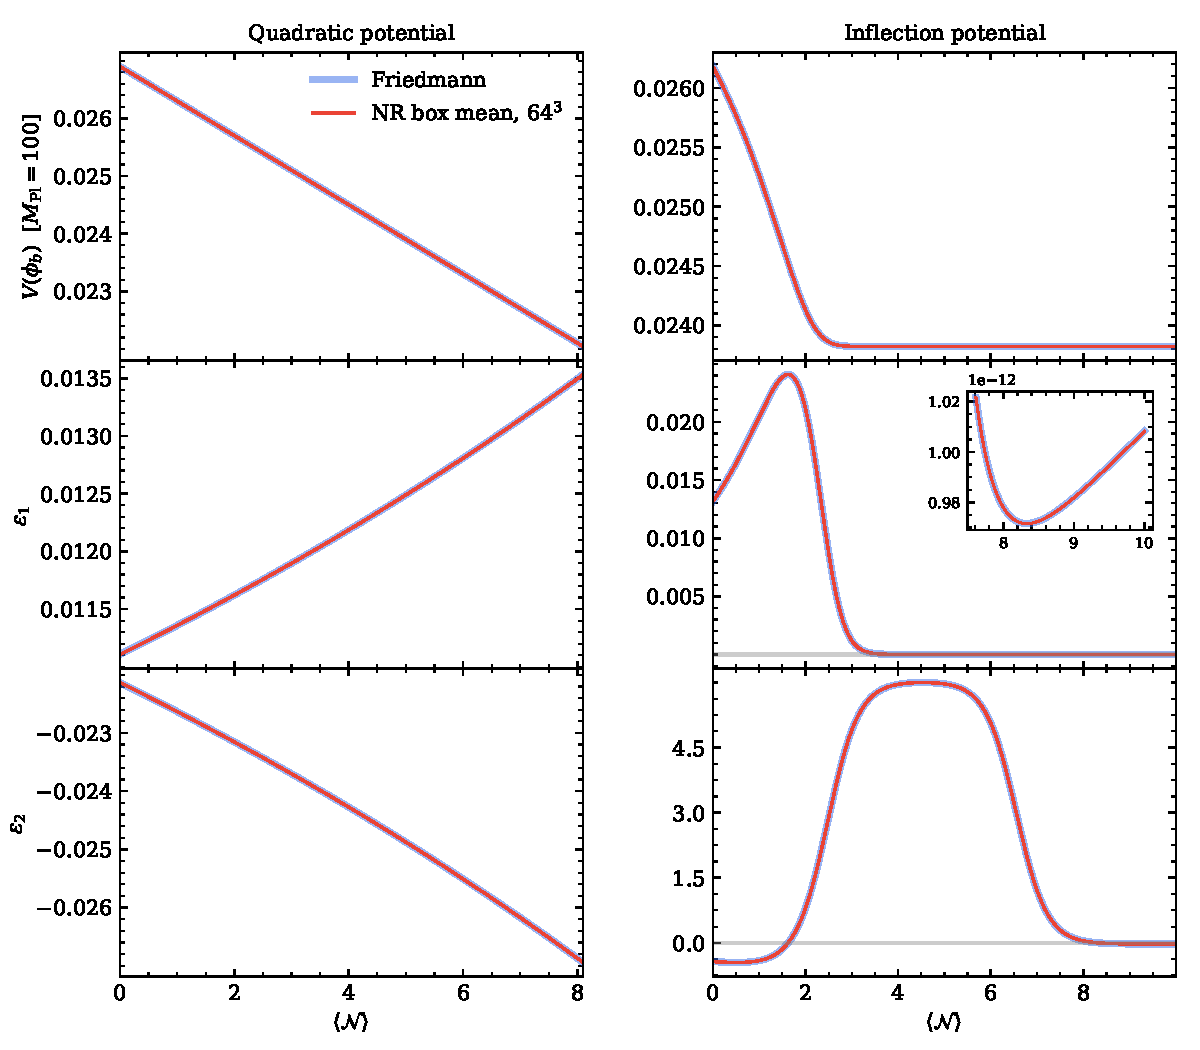
\includegraphics[width=\columnwidth]{fig_background}
\caption{The background of both scenarios. Rows: potential, $\epsilon_1$ and $\epsilon_2$ against the mean number of e-folds. Thick blue: Friedmann solution; thin red: box means of a $64^3$ lattice run. The inset magnifies the minimum of $\epsilon_1$ after the plateau.}
\label{fig:background}
\end{figure}

\subsection{Spectra of the curvature perturbation}\label{sec:spectra}

As the window passes a mode, its power on the lattice rises from the vacuum spectrum to the Mukhanov--Sasaki spectrum and stops changing (Figs.~\ref{fig:specsr} and \ref{fig:specusr}). In SR the final spectrum is flat; in USR it rises with $k$ to order unity at the cut-off, the level \Ptwo{} reports. At the end of the run every shell agrees with the linear power of the same realization; the remaining departure grows toward the cut-off, where difference (c) and, in USR, the second order at order-unity power act. Above the cut-off the USR spectrum shows a second-order shelf, as in \Ptwo{}'s figure. The published spectra and ours agree in level at every time we can compare.

\begin{figure*}
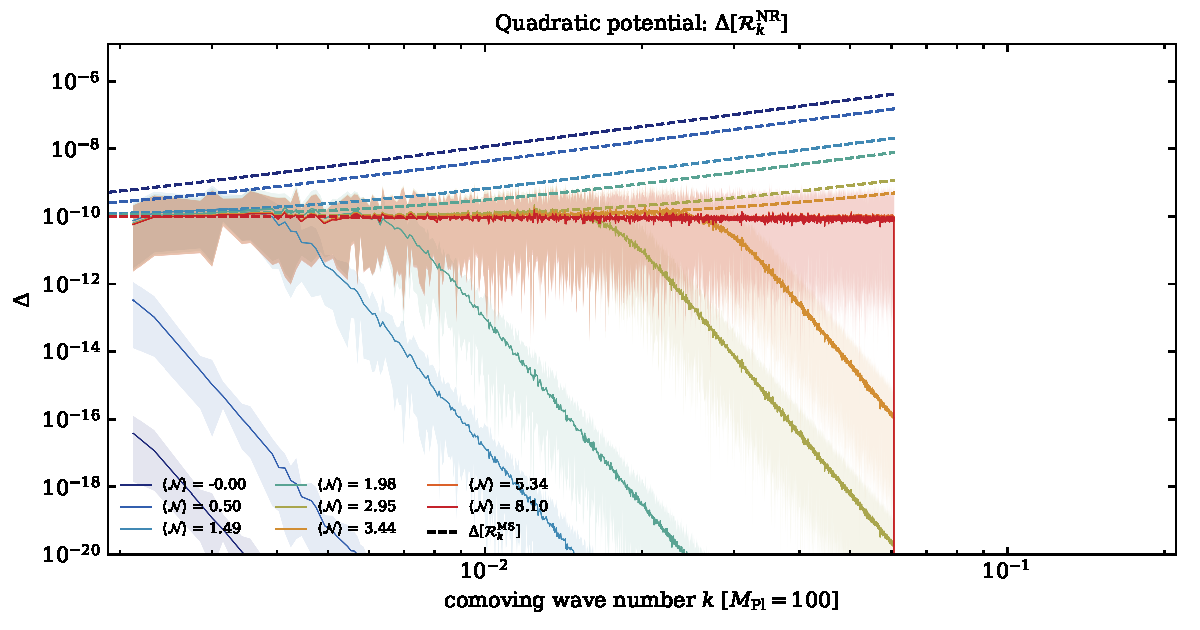
\includegraphics[width=0.85\textwidth]{fig_spec_sr}
\caption{Spectrum of the curvature perturbation on the $256^3$ SR lattice from the start to the end of the run (solid), with the Mukhanov--Sasaki expectation (dashed). Bands: range of the power within each shell. Colors run from early (blue) to late (red) mean e-folds.}
\label{fig:specsr}
\end{figure*}

\begin{figure*}
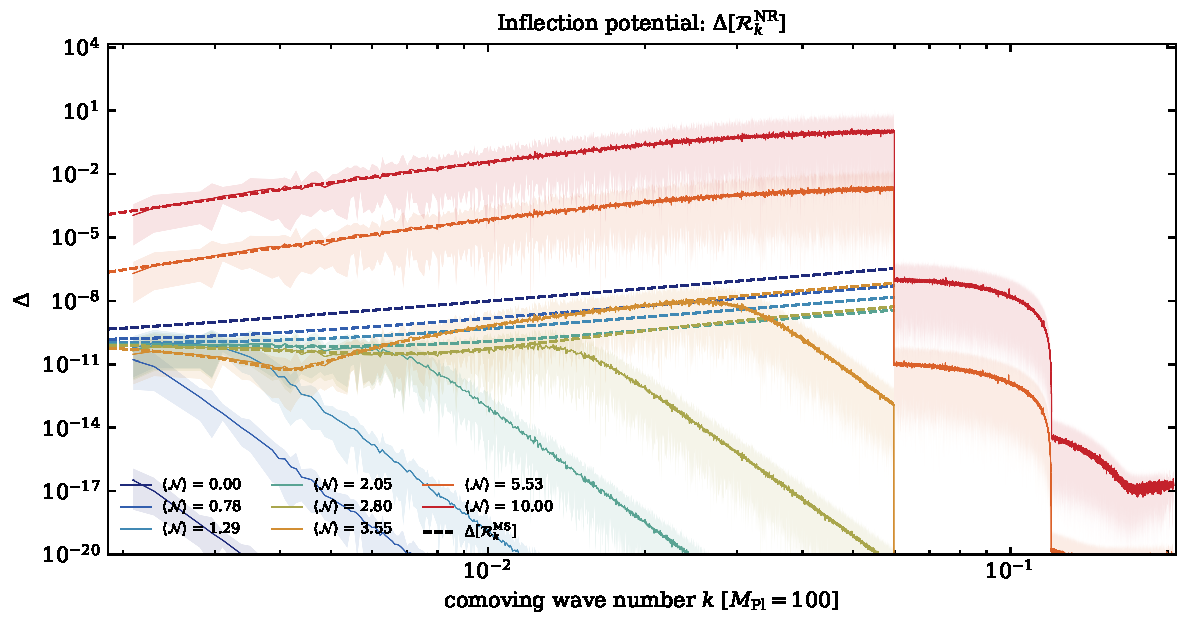
\includegraphics[width=0.85\textwidth]{fig_spec_usr}
\caption{As Fig.~\ref{fig:specsr} for the USR lattice. The late spectra rise toward the cut-off; above it a shelf of second order in the noise appears.}
\label{fig:specusr}
\end{figure*}

\subsection{One-point statistics: the amplitude factor}\label{sec:onepoint}

The spread of the fields over the lattice cells follows the physics of the entry (Fig.~\ref{fig:contrasts}). In SR the contrasts of $\phi$, $K$ and $\mathcal{R}^\mathrm{NR}$ widen while the modes enter, over the span \Ptwo{} quotes, and freeze; the momentum contrast collapses after the last crossing. In USR the field contrast shows \Ptwo{}'s double feature: it grows, decays while the plateau damps the field velocity, and grows again. The $K$ contrast decays without a second growth, the momentum contrast becomes large at late times, and $\mathcal{R}^\mathrm{NR}$ grows through the USR phase and freezes.

The widths of these bands differ. In both scenarios the published bands are three to four times wider than ours, for every field, while the published spectra agree with ours. For a Gaussian field the one-point variance is fixed by the spectrum,
\begin{equation}
\langle \mathcal{R}^2\rangle = \int \Delta(k)\, \dd \ln k ,
\label{eq:variance}
\end{equation}
and our bands obey this relation for the realization's own spectrum. A published width of the USR curvature perturbation would need a spectrum about fifteen times higher at the cut-off than the published spectrum shows. The factor therefore sits in the normalization of the published real-space draw or in its plotting, which \Ptwo{} does not state, and none of the five set-up differences changes a linear amplitude by a factor of three. We call it the amplitude factor. The independent check read the published figures afresh and found the same factor, about 3.5 in SR and about 4 in USR, and the same agreement of the published spectrum with ours. The amplitude factor also explains the published statement that the furthest outliers of the USR curvature perturbation reach order ten: ours stay several times lower. The published figure itself reaches about 18, so its text and its figure differ by a factor of two as well.

\begin{figure*}
\centering
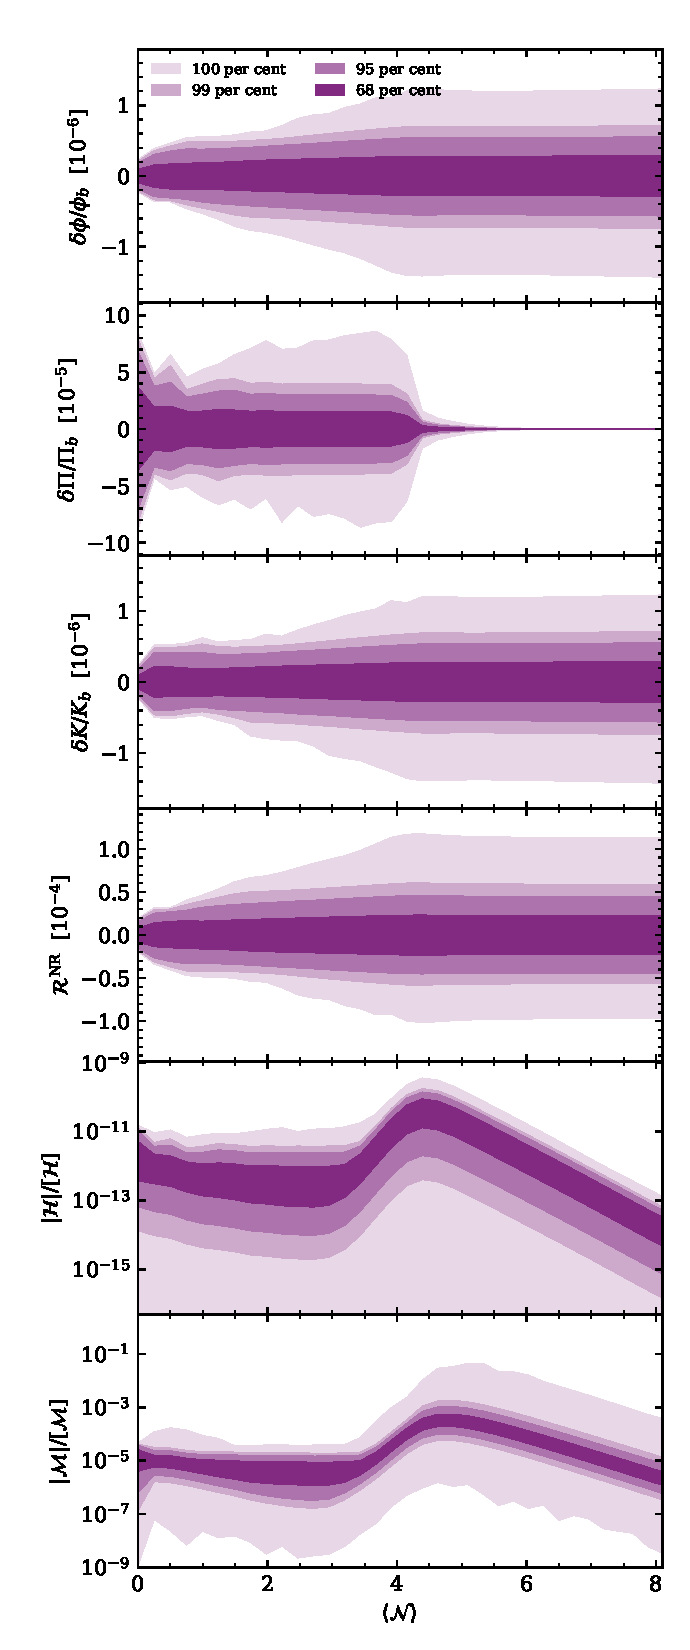
\includegraphics[width=0.34\textwidth]{fig_contrast_sr}\hspace{0.05\textwidth}
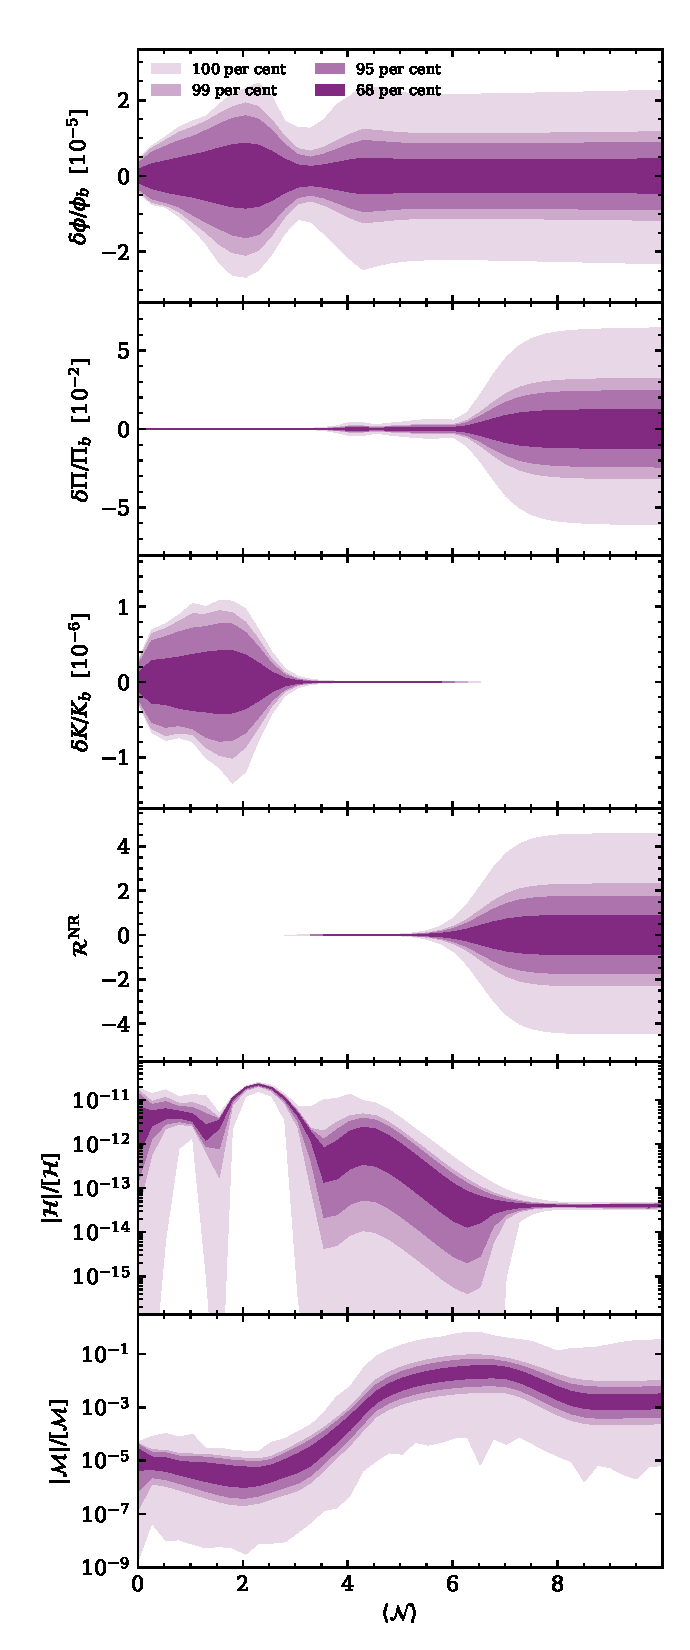
\includegraphics[width=0.34\textwidth]{fig_contrast_usr}
\caption{Spread of the fields over the cells of the $256^3$ lattices, SR (left) and USR (right). Rows: contrasts of field, momentum and $K$, the curvature perturbation, and the constraint ratios; shades: central 68, 95, 99 and 100 per cent. The constraint rows show the ratio in every cell on logarithmic axes.}
\label{fig:contrasts}
\end{figure*}

\subsection{Anisotropic extrinsic curvature}\label{sec:shear}

The trace-free extrinsic curvature carries the anisotropic expansion that the separate-universe picture drops (Fig.~\ref{fig:kspec}). In SR the power of $K$ freezes after the crossings; the trace-free part $\tilde K_{ij}$ is comparable with $K$ during the crossings and then decays, and its invariant $Q = (3\tilde K_{ij}\tilde K^{ij}/2)^{1/2}$ falls below $K$ on every shell. In USR $K$ decays as well and the anisotropic and isotropic parts stay comparable through the plateau, as \Ptwo{} states. After the plateau the hierarchy returns: $Q$ drops below $K$ again on almost every shell. This happens after the last time \Ptwo{} shows, so its statement that the hierarchy is absent in USR holds over the span of its figure, and the hierarchy returns later.

\begin{figure*}
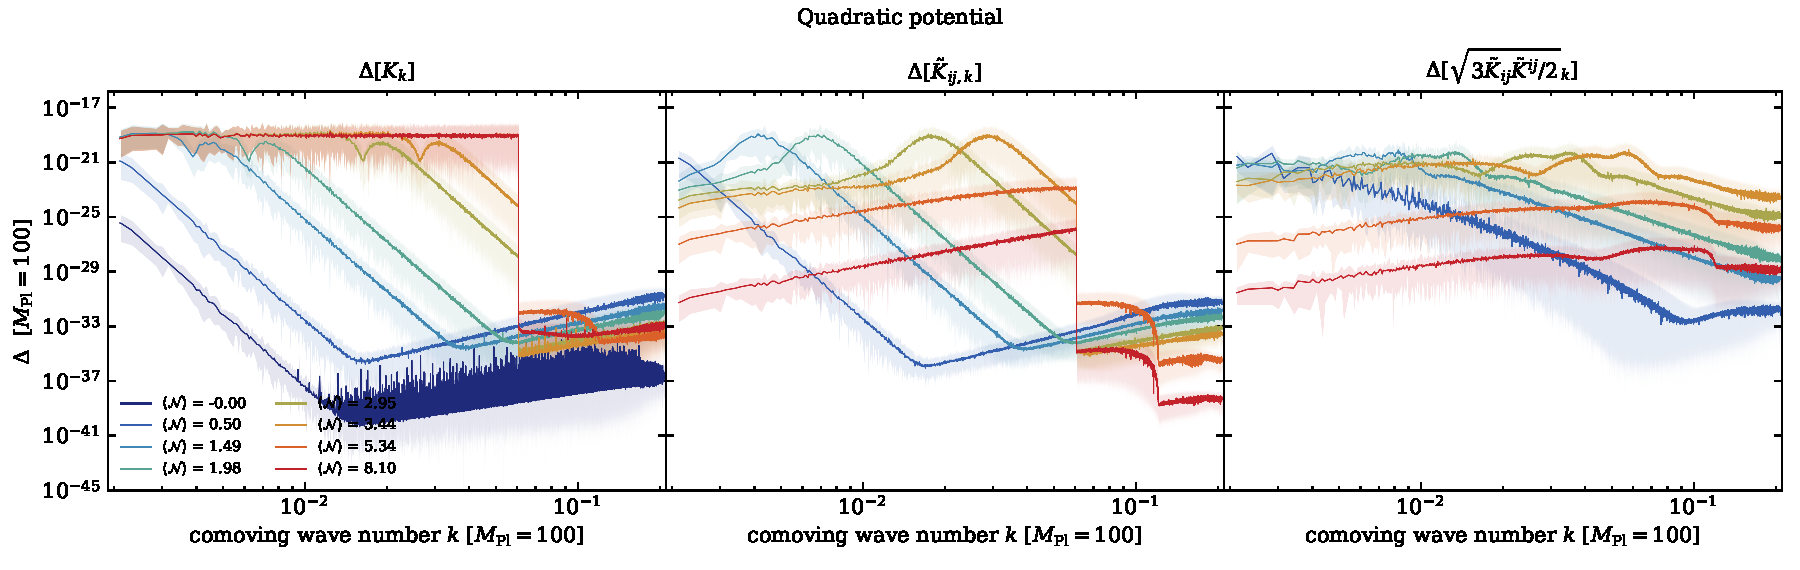
\includegraphics[width=0.85\textwidth]{fig_kspec_sr}\\
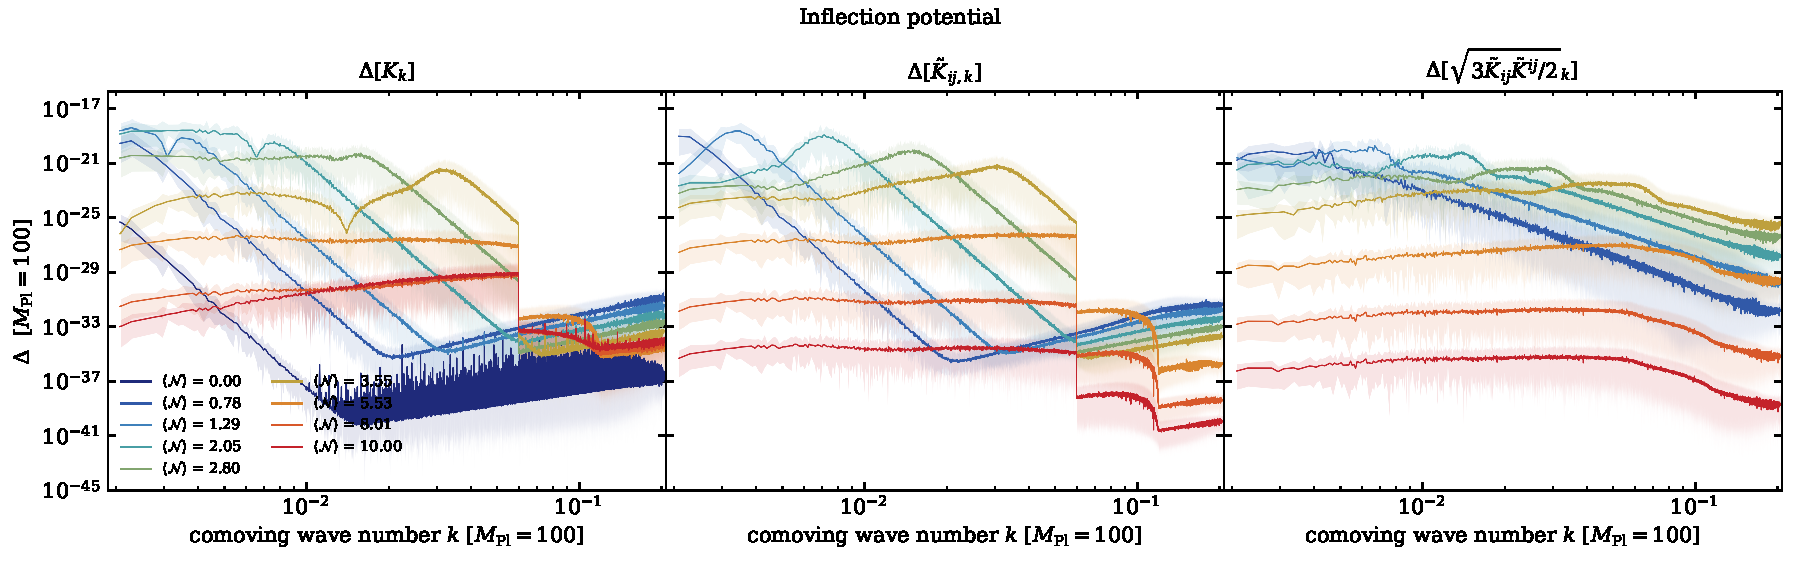
\includegraphics[width=0.85\textwidth]{fig_kspec_usr}
\caption{Spectra of $K$ (left), of the trace-free $\tilde K_{ij}$ (middle) and of $Q$ (right) in units of \Ptwo{}, SR (top) and USR (bottom), from early (blue) to late (red) mean e-folds. Bands: range within each shell.}
\label{fig:kspec}
\end{figure*}

\subsection{Convergence and constraints}\label{sec:constraints}

With the cut-off fixed at eight lattice spacings in wave number, the final spectra converge to the linear spectrum of the realization on all four lattices (Fig.~\ref{fig:specconv}). Up to $128^3$ the largest departure falls by factors of 52 and 62 per doubling, close to the sixth order of the stencils. Against its own continuous-time linear reference the independent check finds factors of 43 and 34, so the measured order lies between five and six and its last digit depends on the reference. From $128^3$ to $256^3$ the largest departure falls by a factor of 2.8, and by 5.8 when $\Phi$ takes the logarithm of $\chi$, the reading of the independent check. There the two finest curves lie on each other at the longest shells, and the scatter of the mode amplitudes about the linear solution is the same on both lattices although the spacing and the step both halve; the independent check finds the two finest fields equal mode by mode to about $10^{-8}$ below $|\bm n| = 4$, thirty times closer than either lies to the linear solution. A floor that ignores the spacing and the step comes from neither the stencils nor the time integrator. Its level depends on the reading at second order: the logarithm moves the modes by $4\times10^{-7}$ in the mean square, on both lattices alike, and halves the scatter about the linear solution. The floor therefore has the size of the second-order terms of the field. Whether it scales with the square of the amplitude, as a second-order term must, a run at half the noise amplitude would show. At shorter scales the finest curve keeps falling. \Ptwo{}'s curves for the two coarser lattices lie where ours do, its two finer curves lie above ours, and its convergence slows as well, which the stencil in its real-space reference can explain.

\begin{figure}
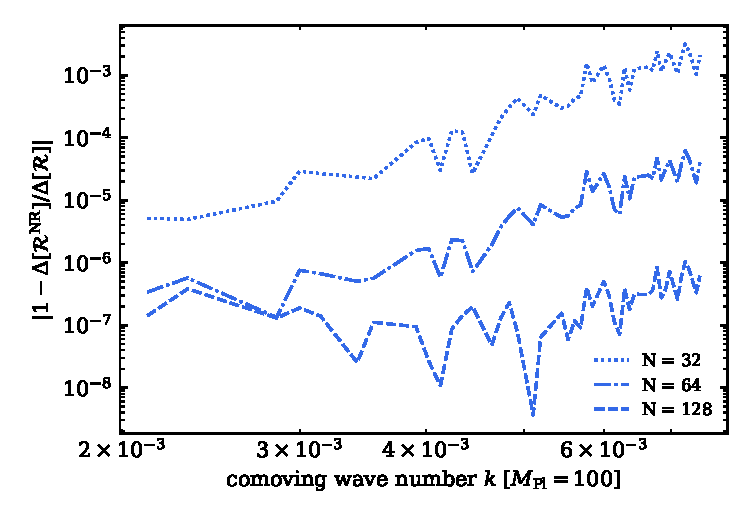
\includegraphics[width=\columnwidth]{fig_specconv}
\caption{Relative departure of the final SR spectrum from the linear spectrum of the same realization, per shell, for four lattices with the cut-off at eight lattice spacings in wave number.}
\label{fig:specconv}
\end{figure}

The constraints show the order of the noise (Fig.~\ref{fig:constraints}). Each kick violates the Hamiltonian constraint at second order, so $\langle|\Ham|/[\Ham]\rangle$ forms a plateau during the entry that does not depend on the resolution once the stencils resolve the modes, and decays once inflation has stretched the modes. On the three finer lattices the plateau ratios of both constraints lie within a fifth of one in both scenarios. The coarsest lattice lies above them by its truncation error during the entry. Late in the runs the finer lattices end higher in three of the curves: the SR momentum ratio and both USR ratios with the box mean kept. \Ptwo{} reports the same for its runs and explains why the test then loses its meaning: the violation reaches a numerical floor sooner, or the plateau amplifies the extra short scales of a finer lattice. Our SR plateau lies between one and two decades below the plateau of \Ptwo{}'s figure, and lower still against the order its text states. The square of the amplitude factor accounts for about one decade, since the violation is quadratic in the amplitude, and the formulation (difference a) can change the level by a factor of order one. Cell by cell, the SR violation reaches the stated order (Fig.~\ref{fig:contrasts}). On the $256^3$ lattice the upper tail of $|\Ham|/[\Ham]$ stays more than a decade below it on the plateau of the entry, climbs to it at the last crossings and then falls by more than three decades by the end of the run. In USR our box mean of the Hamiltonian constraint carries a uniform residual of the background step, which converges at fourth order in the time step on all four lattices; with the box mean removed, our curves have the published shape.

\begin{figure*}
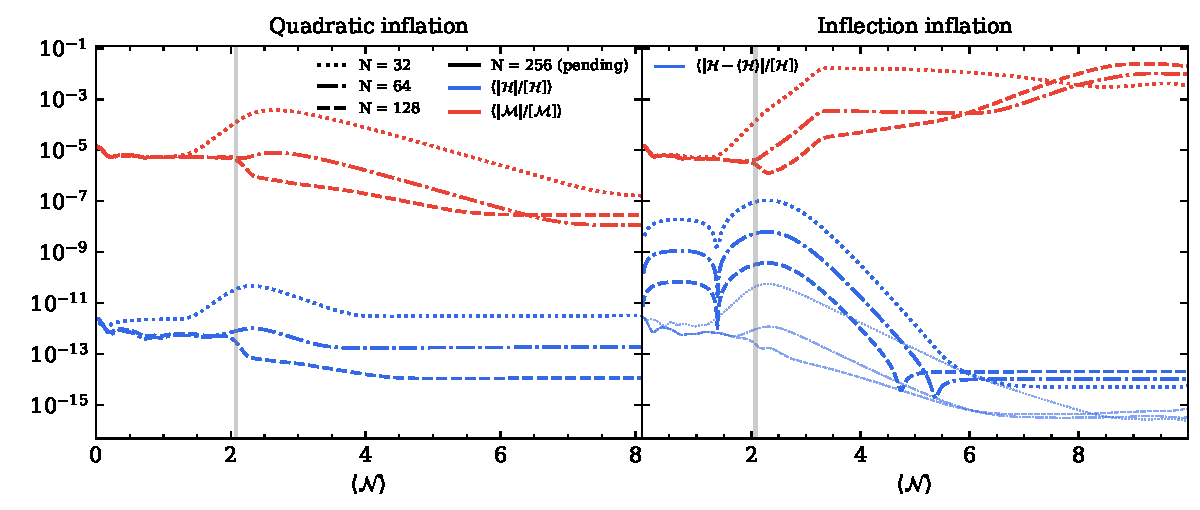
\includegraphics[width=0.85\textwidth]{fig_constraints}
\caption{Constraint ratios against mean e-folds for four lattices with the cut-off at eight spacings: Hamiltonian (blue), momentum (red); thin lines with the box mean of the Hamiltonian constraint removed. Gray line: last crossing at the coarsest lattice.}
\label{fig:constraints}
\end{figure*}

The momentum-constraint magnitude $[\Mom]$ is itself of first order, so a second-order violation gives a ratio of first order. In \Ptwo{}'s set-up the shortest modes enter with four cells per wavelength, and the stencils then add a first-order part to the momentum constraint at the last crossings. \Ptwo{} notes this momentary rise and cures it with a lower cut-off. Our runs show it in the same place, and a scan of the cut-off shows that the first-order part disappears above about thirteen cells per shortest wavelength.

Flipping the sign of the momentum source makes both constraints first order (Fig.~\ref{fig:signflip}), as \Ptwo{} reports. Through the entry of every mode the Hamiltonian ratio of the flipped run lies three to five decades above that of the proper run, and the momentum ratio rises to a sizable fraction of one. Within the entry the gap is smallest at the last crossings, where the violation of the proper run rises; afterwards, by the count of the independent check, it narrows to between two and three decades at the end of the flipped run, as the proper run climbs to the bump of its last crossings and the flipped one decays. The level reached is not the published one. Our flipped Hamiltonian ratio peaks near $10^{-7}$ in both scenarios, a hundred times below the $10^{-5}$ that \Ptwo{} states. The median jump, flipped over proper, is about five decades in SR, the ratio of the two orders \Ptwo{} states, and about four decades in USR, so most of the offset is that of the proper runs above.

\begin{figure}
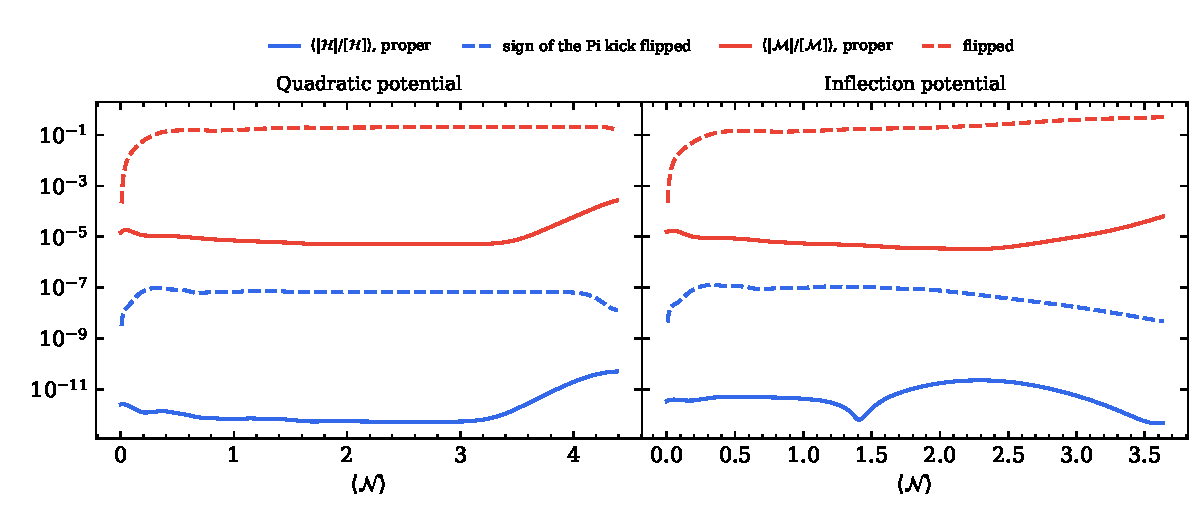
\includegraphics[width=\columnwidth]{fig_signflip}
\caption{Constraint ratios of the proper runs (solid) and of runs with the sign of the momentum source flipped (dashed), SR (left) and USR (right), on $256^3$ lattices.}
\label{fig:signflip}
\end{figure}

\subsection{Stochastic backreaction}\label{sec:backreaction}

\Ptwo{} states that level 2 changes the power by a detectable amount below one part in ten thousand on all scales. To compare levels without difference (c), a development version of the code evolves the noise on the mesh with the lattice gradients at all three levels; a review of its source found no defect in what the runs computed (Appendix~\ref{app:verdicts}). In USR, level 2 against level 0 scatters about zero near one part in ten thousand and rises toward the cut-off, where it exceeds the stated bound (Fig.~\ref{fig:ablation}). \Ptwo{}'s own figure shows the same rise, so its text and its figure disagree and ours follows the figure. The largest shell departs by several parts in ten thousand in our shells and in those of the independent check, which also counts the shells with ten modes or fewer. In SR, level 2 against level 0 is largest on the longest shells and falls toward the cut-off. It stays below the bound on every shell with more than ten independent modes and stops changing once the last mode has crossed: the end of the run repeats the comparison at an earlier time after the last crossing (Fig.~\ref{fig:ablationsr}). The independent check confirms the end of the run with the same shells; counting also the shells with ten modes or fewer, it finds three shells above the bound, all of them sparse, the largest about 1.4 times above it. In SR the comparison therefore sits below the bound on the shells we count and at it on all shells.

Level 1 against level 0 gives a smooth, one-signed difference that grows with $k$, larger than \Ptwo{}'s SR level-1 curve. The review traced it to the two integrations of one background: the level-0 background integrates the Friedmann equation, the mesh evolves $K$ and the conformal factor, and their difference falls by a factor sixteen per halving of the step. The curve therefore measures two fourth-order time integrations of one background, and level 2 against level 0 equals the level-2 effect to a small fraction of itself. The controls of Fig.~\ref{fig:ablation} show why the levels are compared on the mesh: the noise on shells and on the mesh differ at the top shells by the stencil symbol, far above the level-2 effect.

\begin{figure*}
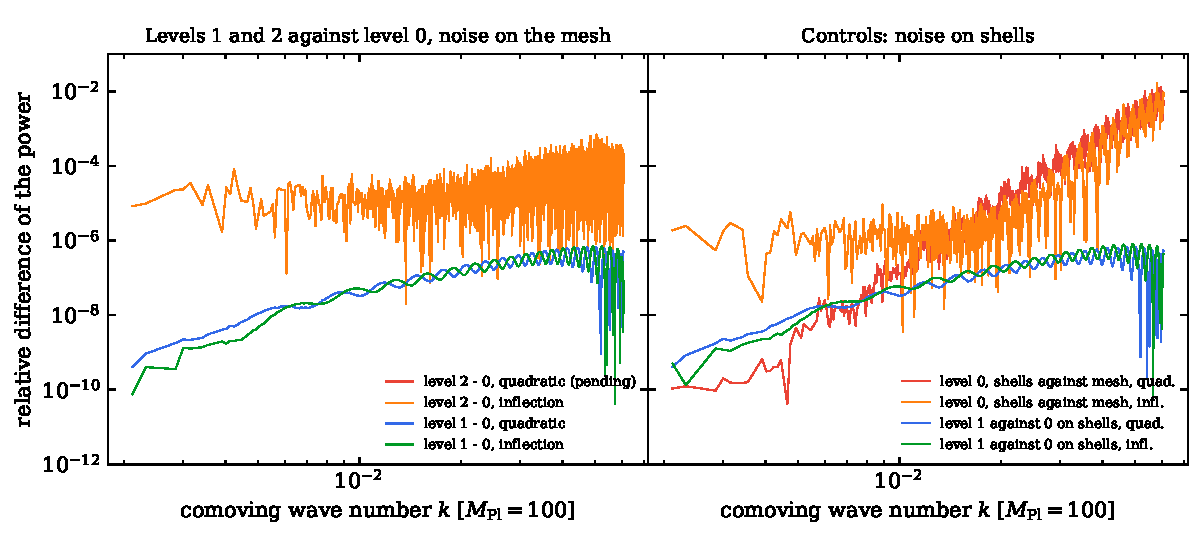
\includegraphics[width=0.85\textwidth]{fig_ablation}
\caption{Relative change of the final power per shell. Left: levels 2 and 1 against level 0, noise on the mesh, SR and USR. Right: controls, noise per shell against noise on the mesh at level 0, and level 1 against level 0 with the noise per shell.}
\label{fig:ablation}
\end{figure*}

\begin{figure}
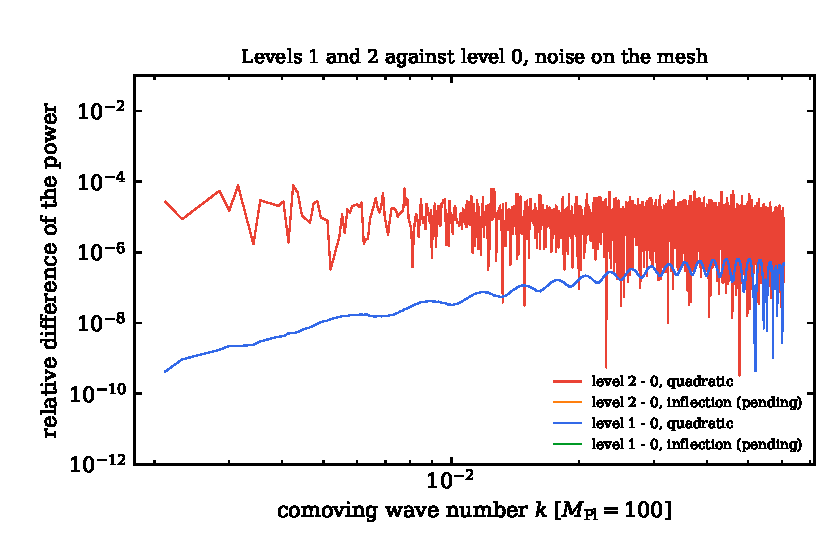
\includegraphics[width=\columnwidth]{fig_ablation_sr}
\caption{As the left panel of Fig.~\ref{fig:ablation} for SR at an earlier time after the last crossing, the time the independent check compared.}
\label{fig:ablationsr}
\end{figure}

\section{The ultra-slow-roll lattice against criteria fixed in advance}\label{sec:criteria}

A reproduction asks whether a code returns what a paper prints. A verified capability asks more: that the code meets thresholds written down before the runs that judge it. For the USR scenario we fixed nine criteria and their thresholds before any production run, together with two rules: maxima run over every record time and every mode, and no record time is dropped afterwards. The criteria cover the background, the linear solution per mode, the freezing of long modes, the constraints, resolution, a second random realization and the coarse-graining window. Figure~\ref{fig:ladder} shows the ladder from these inputs to the outcome, and Table~\ref{tab:ledgerultraslowrollcriteria} of the ledger holds every value.

\begin{figure*}
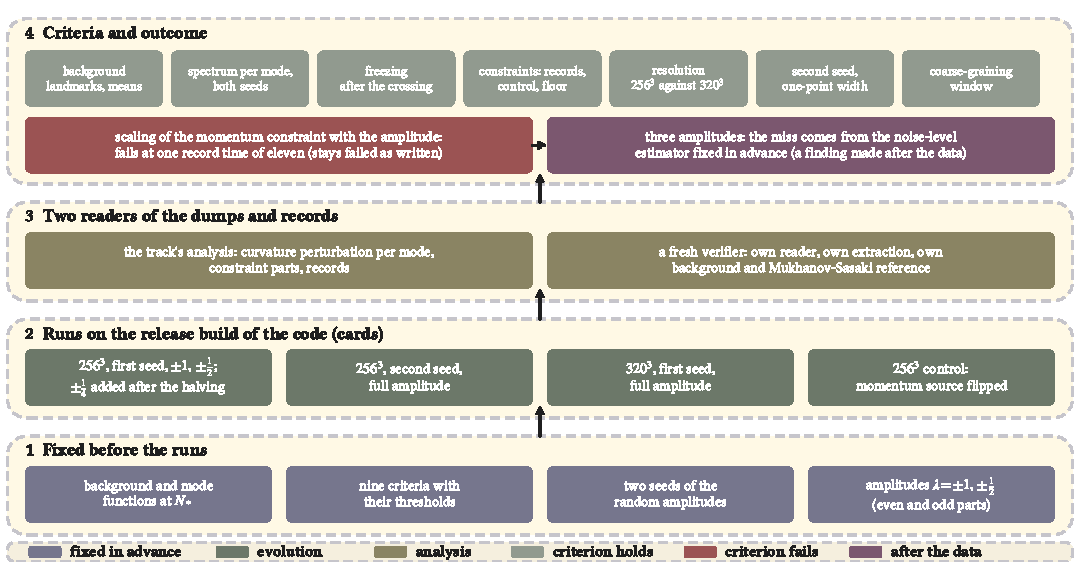
\includegraphics[width=\textwidth]{fig_ladder}
\caption{Verification ladder of the USR lattice, read from the bottom. Inputs and criteria are fixed before the runs; the runs use the release of the code; two independent readers judge the same outputs. Green boxes mark criteria that hold, the red box the one that fails, and the purple box the reading made after the data.}
\label{fig:ladder}
\end{figure*}

\subsection{Runs at several noise amplitudes}\label{sec:amplitudes}

Every stochastic source and the initial slice carry a common amplitude $\lambda$, equal to one in the reproduction. Two runs at $+\lambda$ and $-\lambda$ with the same random numbers split any output $X$ into an odd and an even part,
\begin{equation}
\begin{aligned}
X_\mathrm{odd} &= \tfrac{1}{2}\left[X(\lambda) - X(-\lambda)\right], \\
X_\mathrm{even} &= \tfrac{1}{2}\left[X(\lambda) + X(-\lambda)\right],
\end{aligned}
\label{eq:oddeven}
\end{equation}
which carry the terms of odd and of even order in the noise. Halving $\lambda$ must halve the first-order part of $X_\mathrm{odd}$ and divide the second-order part of $X_\mathrm{even}$ by four. Eleven runs on the release of the code test this. Nine use $256^3$ cells: the first seed at $\lambda = \pm 1, \pm\frac12, \pm\frac14$, a second seed at $\lambda = \pm 1$, and a control with the sign of the momentum source flipped. Two put the first seed at $\lambda = \pm 1$ on $320^3$ cells with the same modes and random numbers. Figure~\ref{fig:mosaic} shows the field the criteria judge: the curvature perturbation at the end of the run, resolved down to the shortest mode of the noise, which spans four cells.

\begin{figure*}
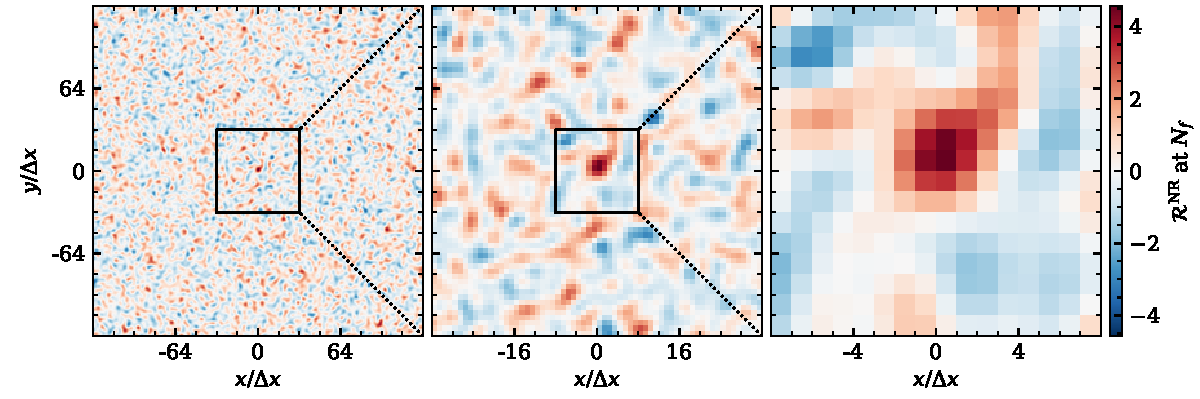
\includegraphics[width=\textwidth]{fig_g2_mosaic}
\caption{Curvature perturbation of the USR lattice at the end of the run, on a slice through its largest value, first seed, $256^3$ cells. Left to right: the whole box, a quarter of its side, and sixteen cells; the black square marks the next panel. Axes count cells from the largest value.}
\label{fig:mosaic}
\end{figure*}

\subsection{Linear agreement, freezing and resolution}\label{sec:linear}

Most criteria hold with wide margins. The box means follow the Friedmann solution, and the background enters and leaves USR at the e-folds of the reference integration. The odd part of the curvature perturbation follows the code's linear mode functions per mode for both seeds, closely up to half the noise cut-off and to the stencil error at the cut-off. The power of the longest modes stays constant after their crossing. The second seed gives the one-point width of the reference lattice. Changing the steepness or the scale of the coarse-graining window moves the shell power far less than the thresholds allow.

The resolution pair behaves as Fig.~\ref{fig:resolution} shows. Above $|\bm n| \approx 25$ the departure per mode falls from $256^3$ to $320^3$ cells by a factor between the fourth-order value $(5/4)^4$ and the sixth-order value $(5/4)^6$, the orders of the time integrator and of the stencils. Below, both lattices share a flat departure that does not depend on the spacing. It is a common factor of all long modes, and the three amplitudes show that it scales as $\lambda^2$: a third-order term of the odd part. The resolution criterion takes the largest departure up to half the cut-off, where this flat part dominates, so it passes with a small margin, and a finer lattice would fail that clause while the discretization error keeps falling.

\begin{figure}
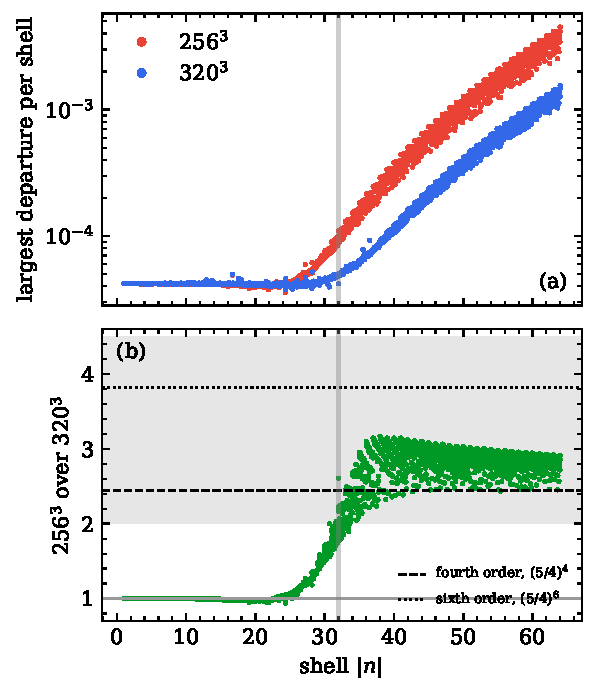
\includegraphics[width=\columnwidth]{fig_g2_resolution}
\caption{Resolution pair of the USR lattice at the end of the run, first seed. (a) Largest departure of the odd part per mode from the linear solution, per lattice shell, on $256^3$ and $320^3$ cells. (b) Their ratio, with the fourth- and sixth-order expectations; the grey band is the range the criterion accepts. The vertical line marks half the noise cut-off.}
\label{fig:resolution}
\end{figure}

\subsection{Second order of the constraints: one failure on record}\label{sec:halving}

The constraint violation of a correct source is second order in the noise, so the even part of each constraint must fall by four when $\lambda$ halves. The criterion compares the root mean square $e(\lambda)$ of the even part over the lattice at each record time. A small part of $e$ does not scale with $\lambda$, so the criterion removes a noise level $f$, estimated as fixed in advance from the odd parts $o$ of the same pair,
\begin{equation}
f^2 = 4\,o(\tfrac12)^2 - o(1)^2 ,
\label{eq:floor}
\end{equation}
and judges every record time at which $e(\frac12)$ exceeds three times $f$. The factor of the Hamiltonian constraint lies in the accepted band at every judged time (Fig.~\ref{fig:halving}a). The factor of the momentum constraint does at every judged time but one, at the end of USR, where it falls below the band (Fig.~\ref{fig:halving}b). As written, this criterion fails, and it stays failed: its estimator was fixed before the runs.

The third amplitude tested whether a fourth-order term in $\lambda$ causes the miss. It does not. From $\lambda = \frac12$ and $\frac14$ the factor at that time lies above four, farther from it than before and on the other side.

\begin{figure}
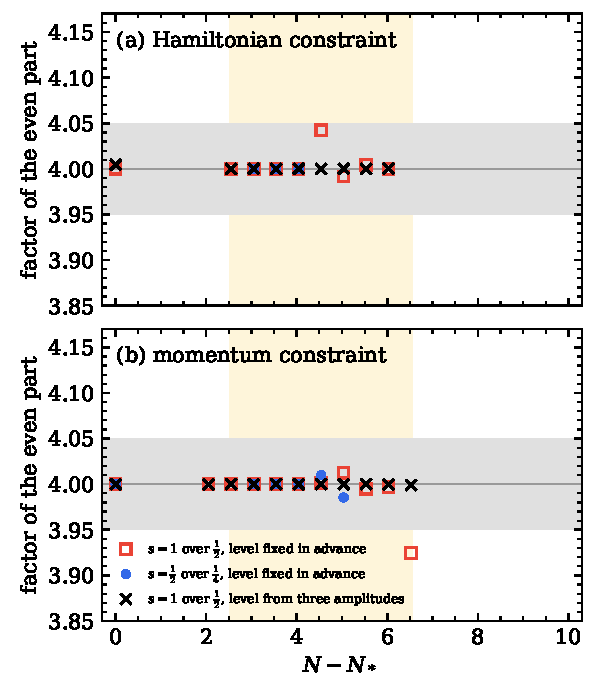
\includegraphics[width=\columnwidth]{fig_g2_halving}
\caption{Factor by which the even part of the Hamiltonian (a) and momentum (b) constraint falls when the noise amplitude halves, at the judged record times. Squares and dots: noise level fixed in advance; crosses: level from three amplitudes. Grey band: accepted range; yellow band: USR.}
\label{fig:halving}
\end{figure}

After the data, the independent check read the three amplitudes together. Write the even field of a constraint as $E(\lambda) = \lambda^2 A + F_\lambda$, where $A$ is the second-order field and $F_\lambda$ a part of each run that does not scale with the amplitude. The two differences
\begin{equation}
D_1 = E(1) - 4E(\tfrac12), \qquad D_2 = E(\tfrac12) - 4E(\tfrac14),
\label{eq:dstat}
\end{equation}
with box means removed, cancel the second-order term. If the parts $F_\lambda$ are independent between runs and of equal size at every amplitude, the two differences have equal size and the correlation
\begin{equation}
\frac{\langle D_1 D_2\rangle}{\sqrt{\langle D_1^2\rangle\langle D_2^2\rangle}} = -\frac{4}{17} ,
\label{eq:corr}
\end{equation}
since only the run at $\lambda = \frac12$ enters both, with weights $-4$ and one. A fourth-order term would instead give a size ratio of $1/16$ and a correlation of one. The measured ratio and correlation match the per-run part at every record time, for both constraints. With the per-run level in place of the estimator fixed in advance, every judged factor lies within a few parts in a thousand of four (crosses in Fig.~\ref{fig:halving}). The fixed estimator subtracts two nearly equal norms of the odd part, which exceeds the even part by one to three decades late in USR, so a third-order term of the odd part moves the estimate by a sizable fraction of itself. The per-run part is deterministic: the release runs repeat earlier runs of a development build bit for bit. We keep this reading beside the failure as a finding made after the data. It changes no verdict.

The constraint records hold their thresholds in every run with the proper source. The control does what a wrong source must: its odd part of the Hamiltonian constraint exceeds that of the proper runs by about five decades through the entry of the modes.

\subsection{Independent check of the criteria}\label{sec:g2check}

A further agent, given the run outputs, the criteria and the predictions but not our verdicts, recomputed every criterion. It wrote its own reader of the dumps and its own extraction of the curvature perturbation, integrated its own background and Mukhanov--Sasaki reference, and drew the random numbers with an independent implementation of the generator. It tested each tool on planted data first. Its values agree with ours to the printed digits for every criterion and for the one failure, and it found no claim wrong. It named three weak points, which this section states: the estimator of the noise level, the resolution clause that measures the flat third-order part, and two clauses whose reading the judge chose (the control counted out of the records criterion, and two readings of the control ratio, both of which pass).

\section{The one-patch reproduction}\label{sec:onepatch}

\subsection{The Langevin pair}\label{sec:langevin}

Without gradients, one coarse-grained patch in the uniform-field gauge carries two variables: its lapse $\alpha$ and its number of e-folds $\mathcal{N}$, both measured against the background e-folds $\mathcal{N}_b$. The Hamiltonian constraint of the patch and its field equation give \Pone{}'s Langevin pair,
\begin{align}
\frac{\partial\mathcal{N}}{\partial\mathcal{N}_b} &= \sqrt{1 + (\alpha^2-1)\left(1-\tfrac{1}{3}\epsilon_1\right)}, \label{eq:lv1}\\
\frac{\partial\alpha}{\partial\mathcal{N}_b} &= 3\alpha\left(\frac{\partial\mathcal{N}}{\partial\mathcal{N}_b} - 1\right) + \alpha^3\langle S^2\rangle \nonumber\\
&\quad + \left(-3+\epsilon_1+\tfrac{1}{2}\epsilon_2\right)\alpha(\alpha^2-1) + \alpha^3 S , \label{eq:lv2}
\end{align}
where $S$ is the noise per e-fold, with the printed amplitude $\langle S^2\rangle^{1/2} = 3H/(2\pi\sqrt{2\epsilon_1}\,\Mpl)$ on the background. The potential is a plateau that joins a cubic slope; the field enters the plateau fast, decelerates in USR, and the noise acts while it crosses the junction (Table~\ref{tab:params}). We integrate the pair with a reference integrator outside the lattice code, in the Stratonovich reading (Heun) and in the It\^o reading (Euler--Maruyama) \cite{Kloeden:1992}, with \Pone{}'s step and number of paths.

\subsection{The background and its step}\label{sec:step}

On a flat plateau the field velocity in e-folds, $\phi' = \dd\phi/\dd\mathcal{N}$, obeys $\phi'' = -(3 - \phi'^2/2)\,\phi'$ in units $\Mpl = 1$, so the velocity decays and the field travels a finite distance. Integrating once gives the plateau stop,
\begin{equation}
\phi_\mathrm{stop} = \phi_* - \frac{1}{\sqrt6}\ln\frac{\sqrt6 + |\phi'_*|}{\sqrt6 - |\phi'_*|},
\label{eq:stop}
\end{equation}
for a field that enters at $\phi_*$ with velocity $\phi'_*$. With \Pone{}'s initial data the plateau stop lies above the junction: the converged background never reaches the slope (Fig.~\ref{fig:lvbackground}). There $\epsilon_1$ keeps falling, the noise amplitude grows as $e^{3\mathcal{N}_b}$, and half the paths blow up before the noise switches off; we count a path as lost once $|\alpha|$ reaches 50 or stops being finite, and the independent check, with its own criterion, finds the half-way point half an e-fold later, still before the switch-off. Forward Euler at \Pone{}'s step of a hundredth of an e-fold overshoots the plateau stop and crosses the junction at the e-fold \Pone{} quotes; Euler at half that step stops short again. \Pone{}'s footnote says that its tuning depends on the step. The published figures are therefore those of the Euler background, and we use it below.

\begin{figure}
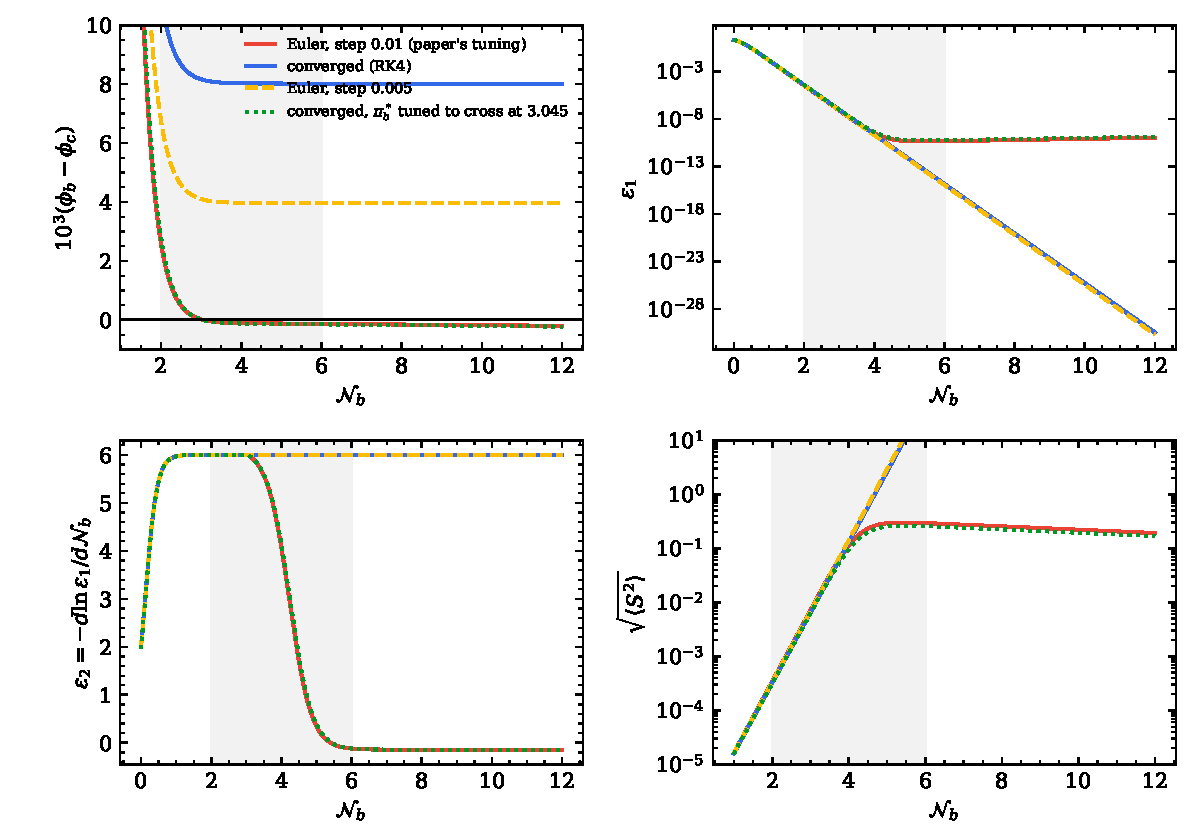
\includegraphics[width=\columnwidth]{fig_lv_background}
\caption{Background of the one-patch system for four integrations: forward Euler at \Pone{}'s step (red) and at half of it (yellow), the converged solution (blue), and a converged solution with the initial velocity tuned to cross (green). Panels: field above the junction, $\epsilon_1$, $\epsilon_2$, noise amplitude. Gray: noise on.}
\label{fig:lvbackground}
\end{figure}

\subsection{Which stochastic reading}\label{sec:reading}

An equation with a noise that multiplies a function of the variable can be read in two ways. The It\^o reading evaluates that function at the start of each step; the Stratonovich reading at its middle. The two differ by a drift equal to half the noise coefficient times its derivative, which here is of the order of the noise variance. \Pone{} names Mathematica's Stratonovich evolver.

On the Euler background, Euler--Maruyama on the printed drift (the It\^o reading) at \Pone{}'s step reproduces the published paths, widths, skewness, kurtosis, distributions and tails (Figs.~\ref{fig:lvpaths}--\ref{fig:lvpdfs}). The independent check integrated the same printed equations with its own code and six seeds: its widths of the lapse and of the e-folds agree with ours and with the published figures to one or two per cent at every record time compared. The third moment is less firm. Our median skewness of the lapse is 1.04, the independent integration gives 1.12, and the published figure about 1.1, so the skewness is reproduced to about ten per cent and depends at that level on details of the integrator. The convergent Stratonovich solution, on which Heun and Euler--Maruyama on the equivalent It\^o drift agree, is wider at late times, more skewed in the lapse, and drifts in $\mathcal{N}-\mathcal{N}_b$ (Fig.~\ref{fig:lvscheme}); at the end of the noise its widths exceed the published ones by 15 to 19 per cent, several times the uncertainty of reading them off. The step of the stochastic integrator alone changes little; the reading decides. At the earliest record time the solution follows the linear covariance of the same background. The data thus point to an Euler-type It\^o integration of the printed drift, against the reading the text names. Only the authors can say which scheme Mathematica applied.

\begin{figure}
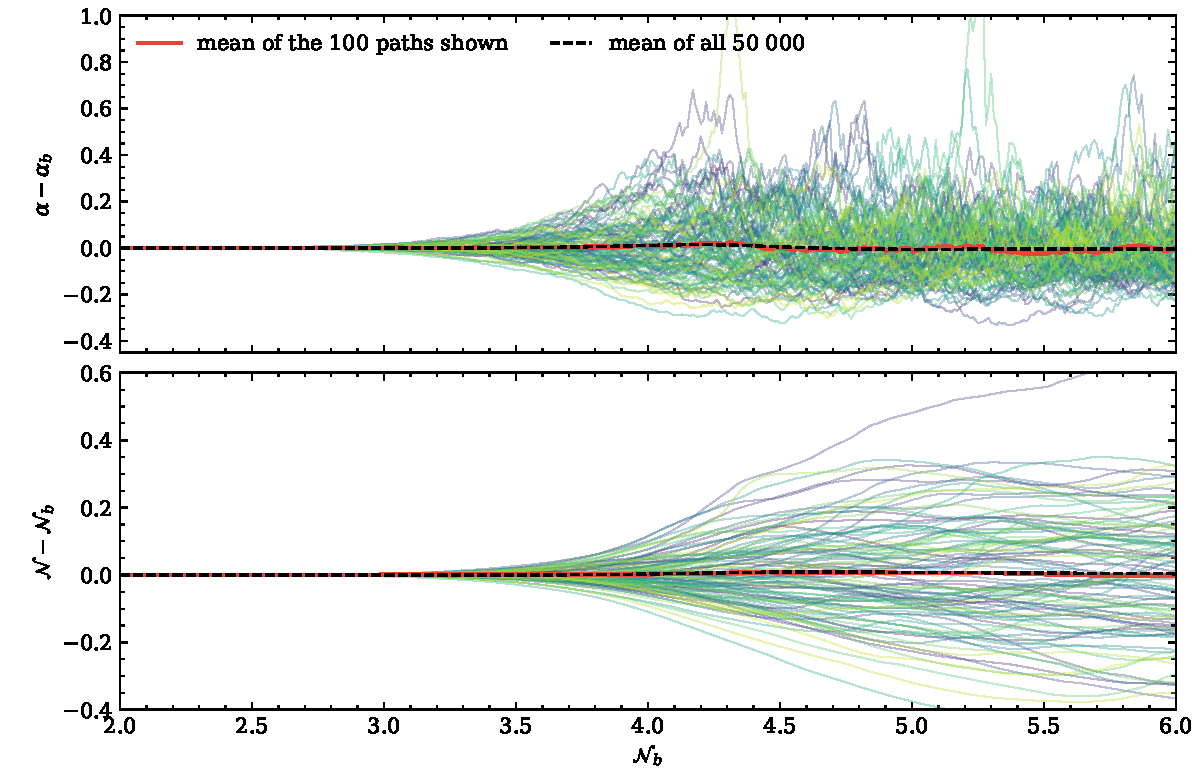
\includegraphics[width=\columnwidth]{fig_lv_paths}
\caption{One hundred paths of the lapse (top) and of the e-folds (bottom) relative to the background, It\^o reading at \Pone{}'s step on the Euler background. Red: mean of the paths shown; black dashed: mean of all paths.}
\label{fig:lvpaths}
\end{figure}

\begin{figure}
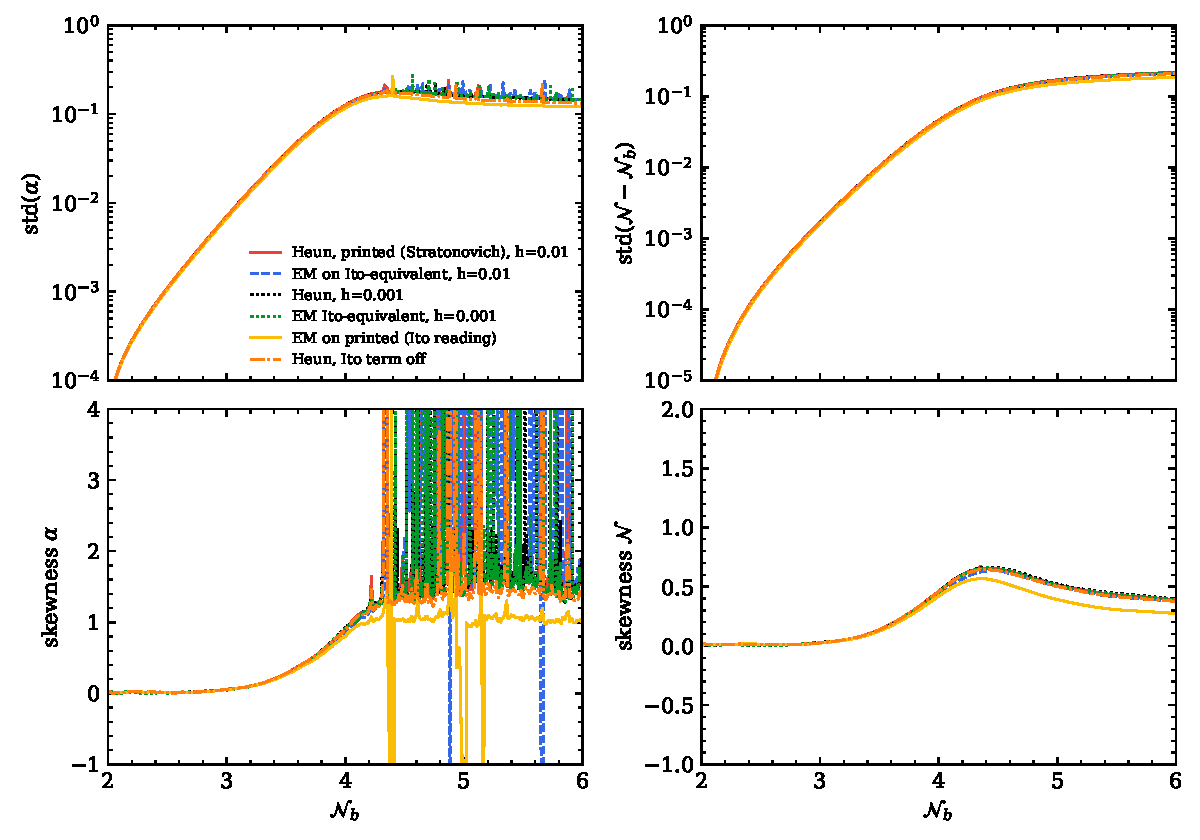
\includegraphics[width=\columnwidth]{fig_lv_scheme}
\caption{Width (top) and skewness (bottom) of the lapse (left) and of the e-folds (right) for six integrations. Yellow: the It\^o reading at \Pone{}'s step; the others are Stratonovich solutions at two steps and the Stratonovich run without the It\^o term.}
\label{fig:lvscheme}
\end{figure}

\begin{figure}
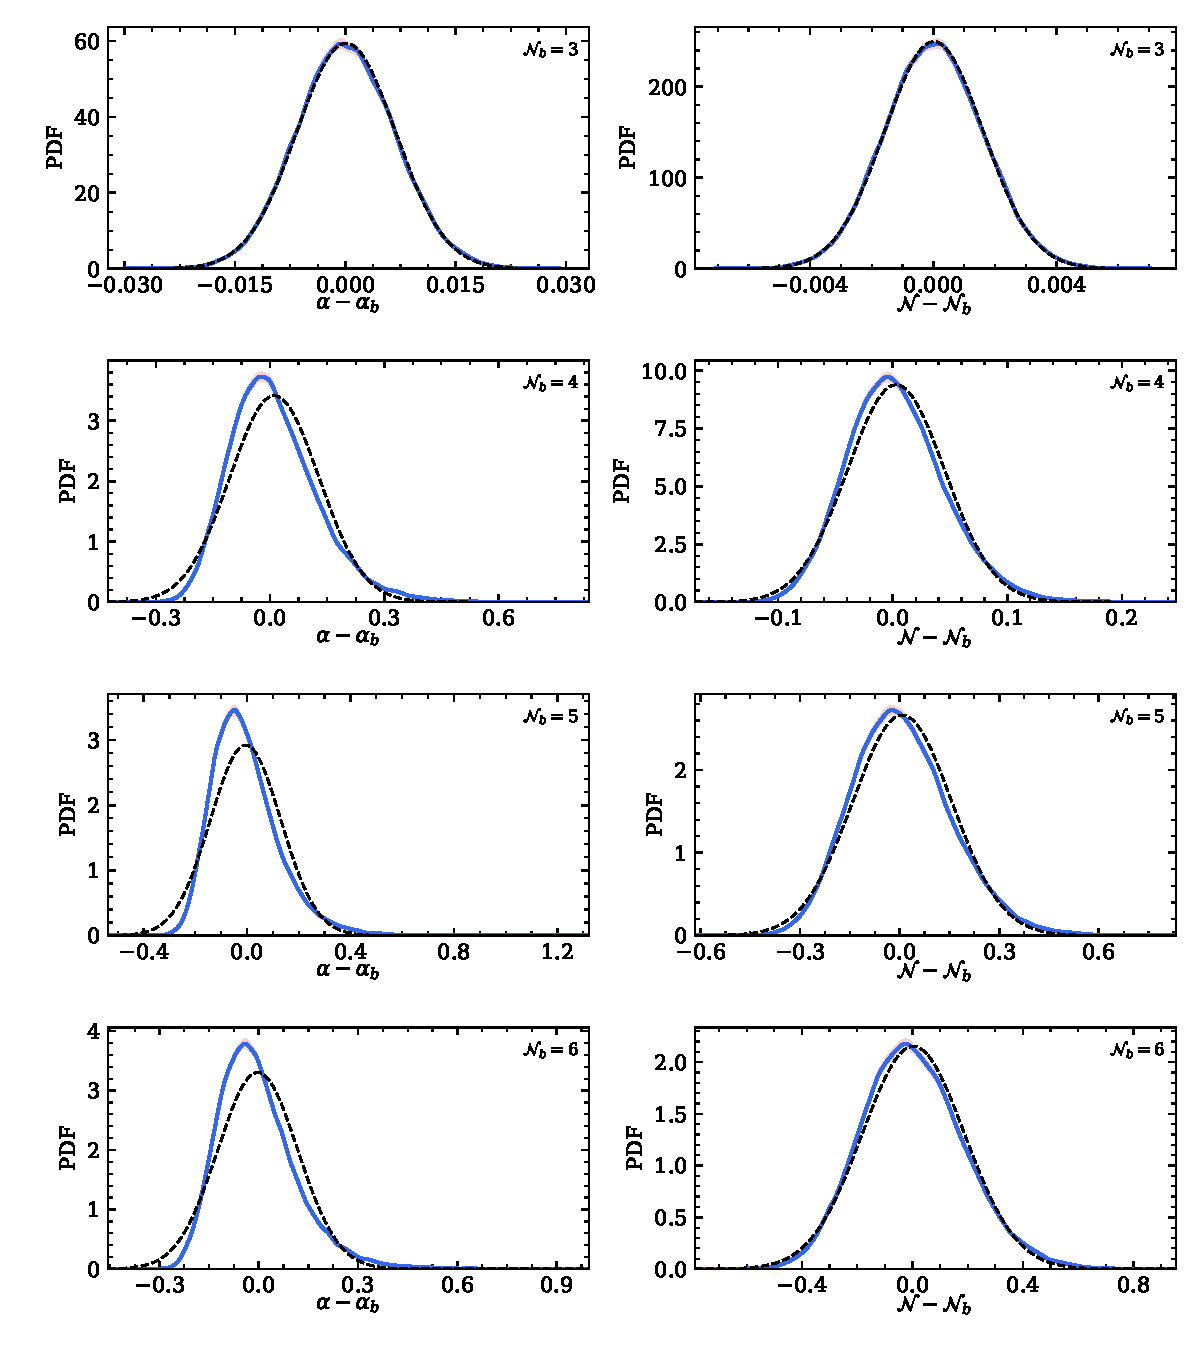
\includegraphics[width=\columnwidth]{fig_lv_pdfs}
\caption{Distributions of the lapse (left) and of the e-folds (right) at four background e-folds, It\^o reading. Blue: kernel estimate with its bootstrap band (light red); dashed: Gaussian of the same mean and width.}
\label{fig:lvpdfs}
\end{figure}

\subsection{The It\^o term and the ultra-slow-roll amplitude}\label{sec:ito}

\Pone{} derives the drift $\alpha^3\langle S^2\rangle$ in the lapse equation with It\^o's lemma. In cosmic time the field equation evolves $Z = \dot\phi_b/\alpha$ with the noise $\alpha S_\Pi$, and the lapse is $\alpha = f(Z) = \dot\phi_b/Z$. It\^o's lemma adds half the second derivative times the noise variance,
\begin{equation}
\frac{1}{2} f''(Z)\,\alpha^2\langle S_\Pi^2\rangle = \frac{\alpha^3}{\dot\phi_b^2}\,\alpha^2\langle S_\Pi^2\rangle = \frac{\alpha^5}{\dot\phi_b^2}\langle S_\Pi^2\rangle ,
\label{eq:itoterm}
\end{equation}
the fifth power of the lapse. The printed third power belongs to a noise $S_\Pi$ without the factor $\alpha$, whose noise term in the lapse equation would carry $\alpha^2$. A Monte Carlo integration of the $Z$ equation confirms the fifth power. The term is small: switching it off moves the widths far less than the choice of reading does.

\Pone{}'s appendix gives the noise amplitude for both SR and USR. Its integration by parts leaves, at the crossing $k = \sigma a H$, the combination $\mathcal{R}' + (3 - \epsilon_1 - \epsilon_2)\mathcal{R}$, with primes for e-fold derivatives. In USR $\epsilon_1$ falls as $a^{-6}$, so $\mathcal{R}' = 3\mathcal{R}$ at leading order and the combination cancels with $\epsilon_2 = 6$. The next order leaves the amplitude smaller than printed by the factor $\sigma^2/3$. The printed value follows only if $\mathcal{R}'$ is dropped. An exact Mukhanov--Sasaki integration in the independent check gives the same factor. In SR the printed amplitude holds up to a correction that grows with $\epsilon_1$ at the crossing: the ratio exceeds one by about $5\epsilon_1$, so it is 1.03 on our background and 1.06 and 1.12 on the two backgrounds of the independent check, whose $\epsilon_1$ at the crossing is larger than ours by factors of about 2.4 and 4.7. The published figures use the printed amplitude, and so does our reproduction of them.

\subsection{The other statements of the text}\label{sec:statements}

Switching the noise off returns the lapse to one and freezes the e-folds, as \Pone{} states. Setting the factor $\alpha^3$ of the noise to one gives left-skewed distributions, as stated, and paths that cross zero lapse; the independent check finds the left skew too, weaker than ours in its single seed. The distribution of the lapse develops an exponential tail after the plateau; that of the e-folds is much heavier than Gaussian and lies between a Gaussian and an exponential tail. Appendix~\ref{app:verdicts} lists each statement with its verdict.

\section{Discussion}\label{sec:discussion}

Everything that linear theory fixes is reproduced on the lattice: the background, the spectra and their freezing, the anisotropic extrinsic curvature through the crossings, the convergence of the spectra, and the order of the constraint violation together with its first-order rise under a flipped source. These quantities test the stochastic sources themselves, and they hold in an independent code with a different formulation, time integrator and random realization.

The departures cluster where a choice enters that the papers do not state. On the lattice it is the normalization of the one-point statistics: the amplitude factor separates the published bands from the published spectra, and through its square it accounts for most of the gap in the constraint levels. In one patch it is the background step and the stochastic reading. Two further departures are statements of a text that its own figure contradicts: the start of USR in \Ptwo{} and its bound on the backreaction at the shortest scales.

The criteria fixed in advance turn the USR lattice into a verified capability with one failure on record. Two of them measure less than they were meant to: the scaling of the momentum constraint rests on an estimator of the noise level that loses its accuracy where the odd part dominates, and the resolution clause reads the flat third-order part of the long modes. Both call for a third amplitude in later tests, which separates the per-run part and the third-order term from the discretization error.

Appendix~\ref{app:verdicts} gives the verdicts. Reproduced: the background, both spectra, the anisotropic curvature, the convergence of the spectra on four lattices, the constraint plateaus, the first-order rise under a flipped sign in both scenarios, and the four figures of \Pone{} in the It\^o reading, whose widths hold to one or two per cent and whose skewness holds to about ten per cent. Reproduced in part: the one-point figures (shape and timing yes, amplitude no), the constraint levels, the level reached under a flipped sign, the bound on the backreaction, the absent hierarchy of the USR shear (true until shortly after the plateau). Not reproduced: the order-ten outliers of the USR curvature perturbation, which follow from the amplitude factor. Open: whether the floor of the spectral convergence at the longest shells of the finest lattice, of the size of the second-order terms, scales with the square of the amplitude.

The independent check confirmed every one of these verdicts from the raw outputs, except for the spectra of the extrinsic curvature, the momentum constraint against the cells per wavelength, the computer-algebra checks of the gauge families and nine of the seventeen misprints, which it did not redo. A second pass of the check took up the continued runs: all five join their originals without a jump, bit for bit where they overlap, and it confirmed the finest lattice of both convergence figures (the digits of the spectral one up to the reading of $\chi$), the end of the SR level-2 run and the SR sign flip over its whole span. Its numbers differ from ours in seventeen of the ledger's rows. In each the difference lies in a definition: the shells counted, the linear reference, the reading of the conformal factor at second order, the sampling of the dumps, the criterion for a lost path, or the implementation of a one-patch integrator for a third moment. None changes a verdict. The shells it counts decide one wording: with them the SR level-2 comparison sits slightly above the published bound, which is why the verdict on the bound reads ``at the bound'' for SR.

\section{Summary}\label{sec:summary}

Five rules come out of the reproduction and the criteria.
\begin{enumerate}
\item An independent numerical-relativity code reproduces the stochastic sources of general relativity, because the sources follow from linear theory and keep the constraints unsourced. Its spectra converge at the order of the stencils down to a floor on the finest lattice, of the size of the second-order terms of the field.
\item A one-point spread must match its spectrum. For a Gaussian field the variance is the integral of the power over the logarithm of the wave number, and the published lattice figures miss it by a factor of three to four.
\item The constraints count the order of the noise: a correct source leaves a second-order violation, a wrong sign a first-order one.
\item A plateau stops a field that is integrated exactly. The published one-patch figures need the coarse Euler step that carries the field over the junction, and the It\^o reading of the printed equation.
\item Two amplitudes cannot separate a part of each run that ignores the amplitude from the scaling of the constraints, because the estimate subtracts two nearly equal norms; three amplitudes can.
\end{enumerate}

Open questions remain physical ones. How does level 2 of the backreaction change the tails of the curvature perturbation, where it acts at second order and the one-point statistics are non-Gaussian? Does the one-patch system, integrated on a background that does reach the slope, keep the exponential tails of the lapse? And how many realizations does a tail statistic in full general relativity need?

\begin{acknowledgments}
The authors of the two reproduced papers made their sources public on the arXiv.
\end{acknowledgments}

\appendix

\section{Misprints}\label{app:errata}

Table~\ref{tab:errata} lists the misprints found by the computer-algebra checks, with the corrected form. None of them changes a run of either paper that we can see; the code follows the corrected forms.

\begin{table*}
\caption{Misprints of \Pone{} and \Ptwo{}, with the corrected form and the check that shows each. The field momentum of the initial slice of Ref.~\cite{Launay:2025bd} needs the same kind of correction and is used corrected. The independent check rederived items 1, 3, 6, 7, 8 and 10 with its own computer algebra and items 14 and 15 with its own derivation, Monte Carlo and Mukhanov--Sasaki integration, and confirmed each.}
\label{tab:errata}
\footnotesize
\begin{tabular}{p{0.04\textwidth}p{0.3\textwidth}p{0.6\textwidth}}
\toprule
& Where & Correct form and check \\
\midrule
1 & linear momentum constraint, both papers & prefactor $-2/3$ (linearization of the nonlinear constraint) \\
2 & linear $K$ equation, \Pone{} & equals the linearized equation up to the linear Hamiltonian constraint; same source \\
3 & nonlinear trace-free equation, both & trace term with $\gamma_{ij}$ in place of $\delta_{ij}$ (else not trace-free for $a \ne 1$) \\
4, 5 & Newtonian gauge, \Pone{} & factor $H$ in $\delta\phi$; one sum for $\Psi$ \\
6 & uniform-$\mathcal{N}$ gauge, \Pone{} & sign of $\delta\mathcal{N}$ from its definition \\
7 & appendix A of \Pone{} & $\ddot H = \epsilon_1(2\epsilon_1+\epsilon_2)H^3$ \\
8 & background relation, \Ptwo{} & $V' = (-3+\epsilon_1+\epsilon_2/2)H\dot\phi_b$ \\
9 & time derivative of the coarse-grained metric potential, \Ptwo{} & $k^2a^{-2}H^{-1}\mathcal{R}$ (dimension) \\
10 & Friedmann line of the usual stochastic equations, both & $H^2 = V/\{3\Mpl^2[1-\pi^2/(6\Mpl^2)]\}$ \\
11 & noise per e-fold, \Pone{} & $\Sigma = H^{-1}\mathcal{F}^{-1}\{S_\Pi\}$ \\
12 & BSSN $K$ equation, both & $-\tfrac{1}{2}\Mpl^{-2}\alpha(\rho+S)$ in a system with $\Mpl$ \\
13 & BSSN momentum constraint, both & sign of the geometric part \\
14 & It\^o term, \Pone{} & $\alpha^5$ (Sec.~\ref{sec:ito}) \\
15 & USR noise amplitude, \Pone{} & smaller by $\sigma^2/3$ (Sec.~\ref{sec:ito}) \\
16 & names of lapse and shift, \Ptwo{} & swapped \\
17 & BSSN trace-free equation, both & one factor $\alpha$ too many in the matter term (our reading) \\
\bottomrule
\end{tabular}
\end{table*}

\section{Scenarios and parameters}\label{app:params}

Table~\ref{tab:params} lists the physical and simulation parameters of both reproductions, as the papers print them and as we set them. Lattice runs use the release version of the code; the comparison of the backreaction levels uses a reviewed development version that adds level 2 and the noise on the mesh.

\begin{table*}
\caption{Parameters. Lattice scenarios of \Ptwo{} and the one-patch scenario of \Pone{}. Units: $\Mpl = 100$ in \Ptwo{}, $\Mpl = 1$ in \Pone{}; our lattice runs use $G = c = 1$, which changes no dimensionless output.}
\label{tab:params}
\footnotesize
\begin{tabular}{p{0.24\textwidth}p{0.34\textwidth}p{0.34\textwidth}}
\toprule
Item & As printed & Ours \\
\midrule
SR potential & $V = m^2\phi^2/2$; $\epsilon_1 = 0.01$, $\epsilon_2 = -0.02$, $H_0 = 10^{-5}\Mpl$ at the Bunch--Davies start & same; $m$ and $\phi_0$ derived by two integrators \\
USR potential & inflection potential of \Ptwo{} Table I; $\Lambda = 1.86\times10^{-6}$, $v = 0.198\,\Mpl$, $\phi_0 = -1.2\,\Mpl$ & same, coded potential equal to the printed one to rounding \\
E-folds, start to run, run to end & about 5 and 8 (SR), about 3 and 10 (USR) & 5 and 8.10 (SR), 3 and 10 (USR) \\
Lattice & $256^3$; $64^3$ for the background; $32^3$ to $256^3$ for convergence & same \\
Box, window & one window wavelength at the start; $\sigma = 1$, $s = 5$ & same \\
Noise cut-off & a quarter of the Nyquist number ($64\,\Delta k$ at $256^3$); $8\,\Delta k$ for convergence & same \\
Gauge, formulation & geodesic slicing; BSSN, damping off; periodic; no dissipation & geodesic slicing; Z4c, damping off; periodic; no dissipation \\
Stencils, time integrator & sixth order; classical RK4; Courant factor not stated & sixth order; low-storage RK4; Courant factor 0.25 \\
Backreaction & level 2 & level 0 (main runs); levels 0, 1, 2 with the noise on the mesh (Sec.~\ref{sec:backreaction}) \\
Random draw & Gaussian, drawn once & Gaussian, drawn once from keyed counters; two seeds \\
\midrule
One-patch potential & $V_0$ above $\phi_c = 9.056$, $V_0(3x^2-2x^3)$ below, $x = \phi/\phi_c$ & same \\
One-patch initial data & $\phi_* = 10$, $\phi'_* = -2.0001$, $H_* = 10^{-5}$ & same; $V_0$ from the Friedmann constraint \\
Noise, paths, step & on for $2 \le \mathcal{N}_b < 6$; fifty thousand paths; step 0.01 e-folds; start $\alpha = 1$, $\mathcal{N} = \mathcal{N}_b$ & same; also steps 0.005, 0.02, 0.001 and four seeds \\
Readings & Stratonovich (named) & Stratonovich (Heun), It\^o (Euler--Maruyama on the printed drift), It\^o equivalent of the Stratonovich reading \\
\bottomrule
\end{tabular}
\end{table*}

\section{The set-up item by item}\label{app:setup}

Table~\ref{tab:setup} compares our lattice set-up with \Ptwo{}'s, item by item, and says what each remaining difference can change.

\begin{table*}
\caption{Set-up of the lattice runs against \Ptwo{}. Verdict: same; equivalent (with the reason); different (with what it can change). The five differences (a)--(e) are those of Sec.~\ref{sec:setup}.}
\label{tab:setup}
\footnotesize
\begin{tabular}{p{0.2\textwidth}p{0.3\textwidth}p{0.44\textwidth}}
\toprule
Item & \Ptwo{} & Ours and verdict \\
\midrule
Potentials, parameters & Table I of \Ptwo{} & same \\
Initial conditions & Bunch--Davies modes evolved to the start of the run & equivalent in USR; (d) different for the highest SR shells, which start later; amplitude correction of order $(aH/k)^2$ \\
E-fold spans & approximate & equivalent: integers chosen, reproduce the background figure \\
Box, modes, window, cut-off & as Table~\ref{tab:params} & same \\
Gauge, boundaries, dissipation & geodesic, periodic, none & same \\
Formulation & BSSN, damping off & (a) different: Z4c, damping off; solutions differ by terms proportional to the constraints, second order in the noise; constraint levels can change by factors of order one \\
Stencils & sixth order & same \\
Time integrator & classical RK4 & equivalent: low-storage RK4, fourth order measured with the sources on \\
Step & not stated & Courant factor 0.25; time error far below the reproduced quantities \\
Units & $\Mpl = 100$ & equivalent: dimensionless outputs unchanged \\
Backreaction & level 2 & (b) different: level 0; tested in Sec.~\ref{sec:backreaction} \\
Mode equation of the noise & real space with lattice gradients & (c) different: per shell with the continuum $k$; top shells differ by the stencil symbol \\
Level-0 background & not stated & (e) different: Friedmann lockstep; the mesh evolves $K$ and the conformal factor \\
Initial slice & coarse-grained data of Ref.~\cite{Launay:2025bd} & equivalent: same linear data, corrected field momentum \\
Sources per step & step integral or stage values (both described) & equivalent: stage values, fourth order for frozen amplitudes \\
Sources & $S_\Pi$, $S_K$, $S_{\tilde A_{ij}}$ & same for $\Pi$ and $K$; equivalent for $\tilde A_{ij}$ (projector with the stencil wave number) \\
Extraction of $\mathcal{R}^\mathrm{NR}$ & from conformal factor, metric and field & same at linear order \\
Constraint magnitudes & sums of term magnitudes & same for $[\Ham]$; equivalent for $[\Mom]$ \\
Spectra & shells with more than ten modes & same \\
\bottomrule
\end{tabular}
\end{table*}

\section{Verdicts}\label{app:verdicts}

Table~\ref{tab:verdicts} gives the verdict on each figure and on the quantitative statements of both papers that we tested, with the independent check where there is one. The numbers behind each verdict are in the ledger (Appendix~\ref{app:ledger}).

\begin{table*}
\caption{Verdicts on the figures and statements of both papers. Reproduced, in part, or not reproduced. Check: the verdict of the independent check, which recomputed the claim from the raw outputs with its own code and did not see our conclusions; ``not redone'' marks a claim it reproduced only by rerunning our scripts or did not take up. Its numbers are in the Check column of the ledger.}
\label{tab:verdicts}
\footnotesize
\begin{tabular}{p{0.24\textwidth}p{0.38\textwidth}p{0.32\textwidth}}
\toprule
Item & Verdict & Check \\
\midrule
\Ptwo{} Fig.~1, background & reproduced (Fig.~\ref{fig:background}) & confirmed; two $\epsilon_2$ maxima beyond its reach \\
\Ptwo{} Figs.~2 and 4, one-point statistics & in part: shape and timing yes, constraint rows included; bands narrower by the amplitude factor & confirmed, the factor (about 3.5 in SR, 4 in USR) from its own reading of the published figures; cause open; SR run joined to its end, its constraint rows not recomputed \\
\Ptwo{} Figs.~3 and 5, spectra & reproduced (Figs.~\ref{fig:specsr}, \ref{fig:specusr}) & confirmed per mode and per shell; largest departures 10 to 15 per cent apart (its own linear reference) \\
\Ptwo{} Fig.~6, $K$ and shear spectra & reproduced; absent USR hierarchy in part (returns after the plateau) & not redone \\
\Ptwo{} Fig.~7, spectral convergence & reproduced: four lattices, monotone; order between five and six up to $128^3$, a floor at the longest shells of $256^3$ of the size of the second-order terms & confirmed on four lattices against the code's linear record; floor confirmed, independent of spacing, step and reference; its $256^3$ digits differ by the reading of $\chi$ \\
\Ptwo{} Fig.~8, constraint convergence & in part: plateaus equal on the three finer lattices, decay; levels lower & records, entry maxima and plateau ratios confirmed on four lattices with the stated window; constraint field not recomputed from the metric \\
\Ptwo{} Fig.~9, backreaction & in part: USR level 2 as the figure; SR level 2 unchanged after the last crossing; level 1 is a scheme difference & review of the code: runs stand; values confirmed after the last crossing and at the end of the run, with our shells \\
\Ptwo{}: start of USR & reproduced as the figure shows it; the text is about one e-fold late & confirmed \\
\Ptwo{}: power up to order unity, agreement with linear theory & reproduced & confirmed \\
\Ptwo{}: outliers of order ten & not reproduced (amplitude factor) & confirmed; the published figure reaches about 18 \\
\Ptwo{}: Hamiltonian violation at the next order & in part: second order and damped in both scenarios; per cell on $256^3$ the SR tail reaches the stated order at the last crossings and the USR tail stays a few times lower; box-mean plateaus one to two decades lower & records confirmed from the dumps, to the end of the SR run; constraint field and per-cell tails not recomputed \\
\Ptwo{}: flipped sign gives first order & in part: first order reproduced in both scenarios through the entry; level a hundred times lower than printed & confirmed, including the level, over the whole SR flipped run \\
\Ptwo{}: momentum constraint at the last crossing & reproduced: first-order part below about thirteen cells per wavelength & not redone \\
\Ptwo{}: backreaction below one part in ten thousand & in part: holds at large scales, fails at the USR top shells; SR at the bound & review of the code: runs stand; values confirmed; USR above the bound on a quarter of all shells \\
\midrule
\Pone{} Fig.~1, paths & reproduced in the It\^o reading on the Euler background & confirmed (background and widths) \\
\Pone{} Fig.~2, skewness and kurtosis & reproduced in the It\^o reading, skewness to about ten per cent; in part in the Stratonovich reading & widths confirmed; skewness 1.12 against our 1.04 \\
\Pone{} Figs.~3 and 4, distributions & reproduced in the It\^o reading & confirmed (widths and means) \\
\Pone{}: slope reached near the quoted e-fold & reproduced only with Euler at the printed step & confirmed, with the plateau stop in closed form \\
\Pone{}: Stratonovich evolver & not matched: the figures follow the It\^o reading & confirmed: the Stratonovich widths miss by 15 to 19 per cent \\
\Pone{}: It\^o term $\alpha^3\langle S^2\rangle$ & corrected: $\alpha^5$ (computer algebra and Monte Carlo) & confirmed (derivation and Monte Carlo) \\
\Pone{}: amplitude valid in SR and USR & USR smaller by $\sigma^2/3$; SR close to one, with a correction that grows with $\epsilon_1$ & USR confirmed; SR 1.06 and 1.12 on its backgrounds \\
\Pone{}: noise off, $\alpha^3$ set to one, exponential tails & reproduced; tails of the e-folds in part & left skew confirmed (one seed); tails not redone \\
\bottomrule
\end{tabular}
\end{table*}

\section{Ledger}\label{app:ledger}

Tables~\ref{tab:ledgerlatticebackground}--\ref{tab:ledgerultraslowrollcriteria} list every number behind the text with its source: a registered run of the program, a committed line of its records (for values read off the published figures and for the code review), or a line of a paper's source. A script builds them from the outputs of one registered run and stops if a quoted line has moved. The caption of each table states the definitions behind its rows.

The Check column gives the verdict of the independent check on each row, with the line of its report in brackets: ``yes'', its value agrees within the stated or sampling precision (its value follows where it differs in the last digit or stands for a definition); ``differs'', its value, given, differs beyond the printed digits while the statement it supports holds; ``beyond reach'', its method cannot reach the printed digits; ``quote'', the printed string was checked at its line; ``rerun only'', it reproduced the row only by rerunning our scripts; ``run joined'', it joined the run and compared its records with the dumps but did not recompute the value; a dash, no check (two rows added after the check, and the slice of Fig.~\ref{fig:mosaic}); ``verifier's run'', a value that only the independent check's own run gives. In the table of the USR criteria the Check column cites the report of the independent check of Sec.~\ref{sec:g2check}. The script stops if the verifier's value does not stand on the line it names.

\begin{table*}
\caption{Ledger, lattice background. Each value with its source: a registered run, a committed line of the program's records, or a line of a paper's source.}
\label{tab:ledgerlatticebackground}
\footnotesize
\begin{tabular}{p{0.36\textwidth}p{0.2\textwidth}p{0.38\textwidth}}
\toprule
Quantity & Value & Source \\
\midrule
SR: largest $|$V/\allowbreak{}V\_F - 1$|$ of the box means (64\^{}3) & 9.8e-13 & this run (E-20261124-180038-4d4651a) from records of E-20261123-020704-2b99463 \\
SR: largest $|$eps1/\allowbreak{}eps1\_F - 1$|$ & 6.3e-12 & this run (E-20261124-180038-4d4651a) from records of E-20261123-020704-2b99463 \\
SR: largest $|$eps2 - eps2\_F$|$ & 2.2e-11 & this run (E-20261124-180038-4d4651a) from records of E-20261123-020704-2b99463 \\
SR: e-folds N\_f - N\_* of the run & 8.099 & this run (E-20261124-180038-4d4651a) from records of E-20261123-020704-2b99463 \\
USR: largest $|$V/\allowbreak{}V\_F - 1$|$ & 1.1e-09 & this run (E-20261124-180038-4d4651a) from records of E-20261123-020704-2b99463 \\
USR: largest $|$eps1/\allowbreak{}eps1\_F - 1$|$ & 4.6e-05 & this run (E-20261124-180038-4d4651a) from records of E-20261123-020704-2b99463 \\
USR: largest $|$eps2 - eps2\_F$|$ & 4.4e-05 & this run (E-20261124-180038-4d4651a) from records of E-20261123-020704-2b99463 \\
USR: eps2 = 3 crossed upward at N & 2.523 & this run (E-20261124-180038-4d4651a) from records of E-20261123-020704-2b99463 \\
USR: eps2 = 3 crossed downward at N & 6.550 & this run (E-20261124-180038-4d4651a) from records of E-20261123-020704-2b99463 \\
USR: eps1 at N\_f & 1.01e-12 & this run (E-20261124-180038-4d4651a) from records of E-20261123-020704-2b99463 \\
USR: eps2 at N\_f & -0.0276 & this run (E-20261124-180038-4d4651a) from records of E-20261123-020704-2b99463 \\
Paper II: USR from N $\sim$ 3.5 & ``From $\mathcal{N} \sim 3.5$ USR starts'' & Paper II, source line 534 \\
Paper II: (eps1, eps2) after the plateau & ``$\left(0,-2.8 \times  10^{-2}\right)$'' & Paper II, source line 534 \\
\bottomrule
\end{tabular}
\end{table*}

\begin{table*}
\caption{Ledger, lattice spectra. Each value with its source: a registered run, a committed line of the program's records, or a line of a paper's source.}
\label{tab:ledgerlatticespectra}
\footnotesize
\begin{tabular}{p{0.36\textwidth}p{0.2\textwidth}p{0.38\textwidth}}
\toprule
Quantity & Value & Source \\
\midrule
SR: largest $|$NR/\allowbreak{}linear - 1$|$ over all shells at N\_f (256\^{}3) & 5.2e-03 & this run (E-20261124-180038-4d4651a) from run E-20261121-202935-31520bc, pass E-20261124-133251-42e8aab \\
SR: the same for k $\le$ k\_max/\allowbreak{}2 & 1.0e-04 & this run (E-20261124-180038-4d4651a) from run E-20261121-202935-31520bc, pass E-20261124-133251-42e8aab \\
SR: fraction of shells within 3/\allowbreak{}sqrt(modes) of the Mukhanov-Sasaki solution & 0.9965 & this run (E-20261124-180038-4d4651a) from run E-20261121-202935-31520bc, pass E-20261124-133251-42e8aab \\
SR: power above k\_max over the Mukhanov-Sasaki power at k\_max & 8.7e-14 & this run (E-20261124-180038-4d4651a) from run E-20261121-202935-31520bc, pass E-20261124-133251-42e8aab \\
USR: largest $|$NR/\allowbreak{}linear - 1$|$ over all shells at N\_f & 5.0e-03 & this run (E-20261124-180038-4d4651a) from run E-20261123-021204-2f573ec, pass E-20261124-130628-6790851 \\
USR: the same for k $\le$ k\_max/\allowbreak{}2 & 3.6e-04 & this run (E-20261124-180038-4d4651a) from run E-20261123-021204-2f573ec, pass E-20261124-130628-6790851 \\
USR: fraction of shells within 3/\allowbreak{}sqrt(modes) of the Mukhanov-Sasaki solution & 0.9965 & this run (E-20261124-180038-4d4651a) from run E-20261123-021204-2f573ec, pass E-20261124-130628-6790851 \\
USR: power above k\_max over the Mukhanov-Sasaki power at k\_max & 1.3e-07 & this run (E-20261124-180038-4d4651a) from run E-20261123-021204-2f573ec, pass E-20261124-130628-6790851 \\
Paper II: USR power reaches & ``$\Delta[{\cal R}]\sim 0.1-1$'' & Paper II, source line 536 \\
\bottomrule
\end{tabular}
\end{table*}

\begin{table*}
\caption{Ledger, one-point statistics. Each value with its source: a registered run, a committed line of the program's records, or a line of a paper's source.}
\label{tab:ledgeronepointstatistics}
\footnotesize
\begin{tabular}{p{0.36\textwidth}p{0.2\textwidth}p{0.38\textwidth}}
\toprule
Quantity & Value & Source \\
\midrule
SR: half-width (68 per cent) of R\^{}NR at N\_f & 2.281e-05 & this run (E-20261124-180038-4d4651a) from run E-20261121-202935-31520bc, pass E-20261124-133251-42e8aab \\
SR: rms of R\^{}NR at N\_f & 2.278e-05 & this run (E-20261124-180038-4d4651a) from run E-20261121-202935-31520bc, pass E-20261124-133251-42e8aab \\
SR: N at which dphi/\allowbreak{}phi\_b reaches 95 per cent of its final width & 3.91 & this run (E-20261124-180038-4d4651a) from run E-20261121-202935-31520bc, pass E-20261124-133251-42e8aab \\
SR: the same for R\^{}NR & 3.44 & this run (E-20261124-180038-4d4651a) from run E-20261121-202935-31520bc, pass E-20261124-133251-42e8aab \\
USR: half-width (68 per cent) of R\^{}NR at N\_f & 0.890 & this run (E-20261124-180038-4d4651a) from run E-20261123-021204-2f573ec, pass E-20261124-130628-6790851 \\
USR: rms of R\^{}NR at N\_f & 0.8945 & this run (E-20261124-180038-4d4651a) from run E-20261123-021204-2f573ec, pass E-20261124-130628-6790851 \\
USR: largest $|$R\^{}NR$|$ over the cells at N\_f & 4.57 & this run (E-20261124-180038-4d4651a) from run E-20261123-021204-2f573ec, pass E-20261124-130628-6790851 \\
USR: half-width of dPi/\allowbreak{}Pi\_b at N\_f & 1.24e-02 & this run (E-20261124-180038-4d4651a) from run E-20261123-021204-2f573ec, pass E-20261124-130628-6790851 \\
Paper II, Fig. 2 read off (SR bands) & about 1.0e-6 & tracks/\allowbreak{}E-stoch-inf/\allowbreak{}repro/\allowbreak{}figs/\allowbreak{}RESULTS.md:69 \\
SR amplitude factor, Paper II over ours & factor of about & tracks/\allowbreak{}E-stoch-inf/\allowbreak{}repro/\allowbreak{}figs/\allowbreak{}RESULTS.md:68 \\
USR amplitude factor, Paper II over ours & by a factor 2.3 to 4 & tracks/\allowbreak{}E-stoch-inf/\allowbreak{}repro/\allowbreak{}figs/\allowbreak{}RESULTS.md:102 \\
Paper II, Fig. 4 read off: 100 per cent band of R\^{}NR & about 18 & tracks/\allowbreak{}E-stoch-inf/\allowbreak{}repro/\allowbreak{}figs/\allowbreak{}RESULTS.md:105 \\
Paper II: furthest outliers of R\^{}NR & ``values of $\sim 10$ for the furthest outliers'' & Paper II, source line 534 \\
\bottomrule
\end{tabular}
\end{table*}

\begin{table*}
\caption{Ledger, constraints. Each value with its source: a registered run, a committed line of the program's records, or a line of a paper's source.}
\label{tab:ledgerconstraints}
\footnotesize
\begin{tabular}{p{0.36\textwidth}p{0.2\textwidth}p{0.38\textwidth}}
\toprule
Quantity & Value & Source \\
\midrule
SR: entry maximum of $<$$|$H$|$/\allowbreak{}[H]$>$, 64\^{}3 & 1.8e-12 & this run (E-20261124-180038-4d4651a) from runs E-20261123-020704-2b99463 (records), pass E-20261124-133251-42e8aab \\
SR: entry maximum of $<$$|$H$|$/\allowbreak{}[H]$>$, 128\^{}3 & 2.0e-12 & this run (E-20261124-180038-4d4651a) from runs E-20261123-020704-2b99463 (records), pass E-20261124-133251-42e8aab \\
SR: entry maximum of $<$$|$M$|$/\allowbreak{}[M]$>$, 128\^{}3 & 1.2e-05 & this run (E-20261124-180038-4d4651a) from runs E-20261123-020704-2b99463 (records), pass E-20261124-133251-42e8aab \\
USR: entry maximum of $<$$|$H$|$/\allowbreak{}[H]$>$, box mean removed, 128\^{}3 & 2.2e-12 & this run (E-20261124-180038-4d4651a) from runs E-20261123-020704-2b99463 (records), pass E-20261124-133251-42e8aab \\
USR: entry maximum of $<$$|$H$|$/\allowbreak{}[H]$>$ with the box mean, 128\^{}3 & 3.2e-10 & this run (E-20261124-180038-4d4651a) from runs E-20261123-020704-2b99463 (records), pass E-20261124-133251-42e8aab \\
USR: order of that maximum, 64 to 128 & 4.05 & this run (E-20261124-180038-4d4651a) from runs E-20261123-020704-2b99463 (records), pass E-20261124-133251-42e8aab \\
USR: largest 99th percentile of $|$H$|$/\allowbreak{}[H] over the cells (256\^{}3) & 2.4e-11 & this run (E-20261124-180038-4d4651a) from run E-20261123-021204-2f573ec, pass E-20261124-130628-6790851 \\
USR: largest record mean of $|$M$|$/\allowbreak{}[M] (256\^{}3) & 2.519e-2 & tracks/\allowbreak{}E-stoch-inf/\allowbreak{}repro/\allowbreak{}figs/\allowbreak{}RESULTS.md:265 \\
Paper II: Hamiltonian violation & ``($\sim 10^{-10}$)'' & Paper II, source line 539 \\
Paper II, Fig. 8a read off: SR plateau of $<$$|$H$|$/\allowbreak{}[H]$>$ & about 2e-11 & tracks/\allowbreak{}E-stoch-inf/\allowbreak{}repro/\allowbreak{}figs/\allowbreak{}RESULTS.md:180 \\
Momentum constraint second order from (cells per shortest wavelength) & at least 12.8 cells & tracks/\allowbreak{}E-stoch-inf/\allowbreak{}a4res/\allowbreak{}README.md:85 \\
Sign flipped, SR: ratio of $<$$|$H$|$/\allowbreak{}[H]$>$ to the proper run & 7.3e+04 & this run (E-20261124-180038-4d4651a) from records of E-20261123-045030-c20bcb3, -035925-8439d79, E-20261122-190341-0419be6, E-20261121-211214-0377aab \\
Sign flipped, SR: largest $<$$|$M$|$/\allowbreak{}[M]$>$ & 0.16 & this run (E-20261124-180038-4d4651a) from records of E-20261123-045030-c20bcb3, -035925-8439d79, E-20261122-190341-0419be6, E-20261121-211214-0377aab \\
Sign flipped, USR: median ratio of $<$$|$H$|$/\allowbreak{}[H]$>$ & 8.0e+03 & this run (E-20261124-180038-4d4651a) from records of E-20261123-045030-c20bcb3, -035925-8439d79, E-20261122-190341-0419be6, E-20261121-211214-0377aab \\
Sign flipped, USR: largest $<$$|$M$|$/\allowbreak{}[M]$>$ & 0.50 & this run (E-20261124-180038-4d4651a) from records of E-20261123-045030-c20bcb3, -035925-8439d79, E-20261122-190341-0419be6, E-20261121-211214-0377aab \\
SR per-cell constraint rows of the one-point figure & \pending{continued run} & continued run E-20261124-130529-da8c917 \\
SR sign flip beyond the first e-fold & \pending{continued run} & continued run E-20261124-130629-61fe0b0 \\
Paper II: a flipped sign gives & ``${\cal H}/[{\cal H}]\sim 10^{-5}$ and  ${\cal M}/[{\cal M}]\sim 1$'' & Paper II, source line 541 \\
\bottomrule
\end{tabular}
\end{table*}

\begin{table*}
\caption{Ledger, extrinsic curvature. Each value with its source: a registered run, a committed line of the program's records, or a line of a paper's source.}
\label{tab:ledgerextrinsiccurvature}
\footnotesize
\begin{tabular}{p{0.36\textwidth}p{0.2\textwidth}p{0.38\textwidth}}
\toprule
Quantity & Value & Source \\
\midrule
SR: Delta[K] at N\_f over N = 5.3 (median over shells) & 0.998 & this run (E-20261124-180038-4d4651a) from run E-20261121-202935-31520bc, pass E-20261124-133251-42e8aab \\
SR: Delta[Kt] at N\_f over N = 4.4 (median) & 2.8e-05 & this run (E-20261124-180038-4d4651a) from run E-20261121-202935-31520bc, pass E-20261124-133251-42e8aab \\
SR: Q/\allowbreak{}K at N\_f (median) & 1.5e-09 & this run (E-20261124-180038-4d4651a) from run E-20261121-202935-31520bc, pass E-20261124-133251-42e8aab \\
USR: Delta[K] at N\_f over its maximum (median) & 1.4e-09 & this run (E-20261124-180038-4d4651a) from run E-20261123-021204-2f573ec, passes E-20261124-130628-6790851, E-20261124-141807-8352509, E-20261124-172949-8b2255b \\
USR: Q/\allowbreak{}K at N\_f (median) & 9.4e-07 & this run (E-20261124-180038-4d4651a) from run E-20261123-021204-2f573ec, passes E-20261124-130628-6790851, E-20261124-141807-8352509, E-20261124-172949-8b2255b \\
USR: shells with Q below K, N = 0.26-3.05 & below 0.2 for 0.26 $\le$ N $\le$ 3.05 & tracks/\allowbreak{}E-stoch-inf/\allowbreak{}repro/\allowbreak{}figs/\allowbreak{}RESULTS.md:152 \\
USR: shells with Q below K from N = 7.27 & 0.98-1.0 from N = 7.27 to N\_f & tracks/\allowbreak{}E-stoch-inf/\allowbreak{}repro/\allowbreak{}figs/\allowbreak{}RESULTS.md:153 \\
\bottomrule
\end{tabular}
\end{table*}

\begin{table*}
\caption{Ledger, convergence. Each value with its source: a registered run, a committed line of the program's records, or a line of a paper's source.}
\label{tab:ledgerconvergence}
\footnotesize
\begin{tabular}{p{0.36\textwidth}p{0.2\textwidth}p{0.38\textwidth}}
\toprule
Quantity & Value & Source \\
\midrule
SR spectra: largest $|$1 - Delta\_NR/\allowbreak{}Delta\_lin$|$, 32\^{}3 & 3.2e-03 & this run (E-20261124-180038-4d4651a) from runs E-20261123-020704-2b99463 (records), pass E-20261124-133251-42e8aab \\
the same, 64\^{}3 & 6.2e-05 & this run (E-20261124-180038-4d4651a) from runs E-20261123-020704-2b99463 (records), pass E-20261124-133251-42e8aab \\
the same, 128\^{}3 & 1.0e-06 & this run (E-20261124-180038-4d4651a) from runs E-20261123-020704-2b99463 (records), pass E-20261124-133251-42e8aab \\
SR: order of the entry maximum of H, 32 to 64 & 4.15 & this run (E-20261124-180038-4d4651a) from runs E-20261123-020704-2b99463 (records), pass E-20261124-133251-42e8aab \\
SR: order of the entry maximum of M, 32 to 64 & 3.25 & this run (E-20261124-180038-4d4651a) from runs E-20261123-020704-2b99463 (records), pass E-20261124-133251-42e8aab \\
256\^{}3 rungs (SR spectra; SR and USR constraints) & \pending{continued run} & continued run E-20261124-130952-4be980b, E-20261124-130711-a5dec67 \\
\bottomrule
\end{tabular}
\end{table*}

\begin{table*}
\caption{Ledger, backreaction. Each value with its source: a registered run, a committed line of the program's records, or a line of a paper's source.}
\label{tab:ledgerbackreaction}
\footnotesize
\begin{tabular}{p{0.36\textwidth}p{0.2\textwidth}p{0.38\textwidth}}
\toprule
Quantity & Value & Source \\
\midrule
USR level 2 against 0: rms over the shells at N\_f & 1.0e-04 & this run (E-20261124-180038-4d4651a) from runs E-20261123-153347-18e7c21, -183822-4abbcae, -164235-49b0945, -192948-348e2e5, -153146-d965002, pass E-20261124-133251-42e8aab \\
USR level 2 against 0: largest shell & 7.0e-04 & this run (E-20261124-180038-4d4651a) from runs E-20261123-153347-18e7c21, -183822-4abbcae, -164235-49b0945, -192948-348e2e5, -153146-d965002, pass E-20261124-133251-42e8aab \\
USR level 2 against 0: fraction of shells positive & 0.52 & this run (E-20261124-180038-4d4651a) from runs E-20261123-153347-18e7c21, -183822-4abbcae, -164235-49b0945, -192948-348e2e5, -153146-d965002, pass E-20261124-133251-42e8aab \\
SR level 2 against 0 at N = 7.19: largest shell & 7.9e-05 & this run (E-20261124-180038-4d4651a) from runs E-20261123-153347-18e7c21, -183822-4abbcae, -152119-38957ba, pass E-20261124-141807-8352509 \\
SR level 2 against 0 at N = 7.19: rms for $|$n$|$ $\le$ 32 & 1.5e-05 & this run (E-20261124-180038-4d4651a) from runs E-20261123-153347-18e7c21, -183822-4abbcae, -152119-38957ba, pass E-20261124-141807-8352509 \\
SR level 2 against 0 at N\_f & \pending{continued run} & continued run E-20261124-131359-49afe29 \\
SR level 1 against 0: largest shell & 6.6e-07 & this run (E-20261124-180038-4d4651a) from runs E-20261123-153347-18e7c21, -183822-4abbcae, -164235-49b0945, -192948-348e2e5, -153146-d965002, pass E-20261124-133251-42e8aab \\
USR level 1 against 0: largest shell & 7.0e-07 & this run (E-20261124-180038-4d4651a) from runs E-20261123-153347-18e7c21, -183822-4abbcae, -164235-49b0945, -192948-348e2e5, -153146-d965002, pass E-20261124-133251-42e8aab \\
level 0, noise on shells against on the mesh: largest SR shell & 1.3e-02 & this run (E-20261124-180038-4d4651a) from runs E-20261123-153347-18e7c21, -183822-4abbcae, -164235-49b0945, -192948-348e2e5, -153146-d965002, pass E-20261124-133251-42e8aab \\
Paper II: bound on level 2 against 0 & ``$\lesssim  1$\textpertenthousand'' & Paper II, source line 520 \\
Review: level 1 against 0 falls per halving of the step by & falls by 16 per halving of the & tracks/\allowbreak{}core/\allowbreak{}outbox/\allowbreak{}20261124T143303Z\_\_to-E-stoch-inf\_\_noise-level2-review-runs-stand.md (branch core/\allowbreak{}noise-level2):41 \\
Review: level 2 against 0 equals the level-2 curve to & the level-2 curve to 1 per cent & tracks/\allowbreak{}core/\allowbreak{}outbox/\allowbreak{}20261124T143303Z\_\_to-E-stoch-inf\_\_noise-level2-review-runs-stand.md (branch core/\allowbreak{}noise-level2):43 \\
\bottomrule
\end{tabular}
\end{table*}

\begin{table*}
\caption{Ledger, one patch. Each value with its source: a registered run, a committed line of the program's records, or a line of a paper's source.}
\label{tab:ledgeronepatch}
\footnotesize
\begin{tabular}{p{0.36\textwidth}p{0.2\textwidth}p{0.38\textwidth}}
\toprule
Quantity & Value & Source \\
\midrule
Euler 0.01 background crosses the junction at N\_b & 3.0435 & this run (E-20261124-180038-4d4651a) from simulation E-20261123-021043-d00a314 \\
converged background: field at N\_b = 12 (the plateau stop) & 9.06402 & this run (E-20261124-180038-4d4651a) from simulation E-20261123-021043-d00a314 \\
junction phi\_c of the potential & phi\_c = 9.056 & tracks/\allowbreak{}E-stoch-inf/\allowbreak{}repro/\allowbreak{}langevin/\allowbreak{}README.md:50 \\
Euler 0.005 background: field at N\_b = 12 & 9.05997 & this run (E-20261124-180038-4d4651a) from simulation E-20261123-021043-d00a314 \\
converged background: half the paths lost by N\_b & 4.80 & this run (E-20261124-180038-4d4651a) from simulation E-20261123-021043-d00a314 \\
Paper I: slope reached at & ``$\simeq 3.04$ efolds'' & Paper I, source line 842 \\
Paper I: step of the scheme & ``$0.01$-efolds steps'' & Paper I, source line 842 \\
Paper I: evolver named & ``Stratonovich evolver'' & Paper I, source line 836 \\
Ito reading, width of alpha at N\_b = 4 & 0.1168 & this run (E-20261124-180038-4d4651a) from simulation E-20261123-021043-d00a314 \\
Ito reading, width of alpha at N\_b = 6 & 0.1207 & this run (E-20261124-180038-4d4651a) from simulation E-20261123-021043-d00a314 \\
Ito reading, width of N - N\_b at N\_b = 6 & 0.1853 & this run (E-20261124-180038-4d4651a) from simulation E-20261123-021043-d00a314 \\
Stratonovich reading, width of alpha at N\_b = 6 & 0.1443 & this run (E-20261124-180038-4d4651a) from simulation E-20261123-021043-d00a314 \\
Stratonovich reading, width of N - N\_b at N\_b = 6 & 0.2171 & this run (E-20261124-180038-4d4651a) from simulation E-20261123-021043-d00a314 \\
Paper I, figures read off: widths of alpha at 4, 5, 6 & 0.117, 0.133, 0.121 & tracks/\allowbreak{}E-stoch-inf/\allowbreak{}repro/\allowbreak{}langevin/\allowbreak{}README.md:77 \\
Paper I, figures read off: widths of N - N\_b at 4, 5, 6 & 0.190 & tracks/\allowbreak{}E-stoch-inf/\allowbreak{}repro/\allowbreak{}langevin/\allowbreak{}README.md:78 \\
Ito reading, median skewness of alpha, N\_b in [4.5, 6] & 1.04 & this run (E-20261124-180038-4d4651a) from simulation E-20261123-021043-d00a314 \\
Stratonovich reading, the same & 1.59 & this run (E-20261124-180038-4d4651a) from simulation E-20261123-021043-d00a314 \\
Paper I, figures read off: skewness of alpha & kappa3(alpha) $\sim$ 1.1 & tracks/\allowbreak{}E-stoch-inf/\allowbreak{}repro/\allowbreak{}langevin/\allowbreak{}README.md:78 \\
Stratonovich reading, mean of N - N\_b at N\_b = 6 & 0.085 & this run (E-20261124-180038-4d4651a) from simulation E-20261123-021043-d00a314 \\
Ito reading, mean of N - N\_b at N\_b = 6 & 0.0034 & this run (E-20261124-180038-4d4651a) from simulation E-20261123-021043-d00a314 \\
Ito reading at step 0.001, width of alpha at N\_b = 4 & 0.1225 & this run (E-20261124-180038-4d4651a) from simulation E-20261123-021043-d00a314 \\
linear check at N\_b = 3: width of alpha, run over linear theory & 1.0021 & this run (E-20261124-180038-4d4651a) from simulation E-20261123-021043-d00a314 \\
alpha\^{}3 set to 1: skewness of alpha at N\_b = 6 & -0.96 & this run (E-20261124-180038-4d4651a) from simulation E-20261123-021043-d00a314 \\
Ito term: drift measured by Monte Carlo & 0.3075 & run E-20261123-022009-a53e7ee \\
Ito term: standard error of that drift & 0.0128 & run E-20261123-022009-a53e7ee \\
Ito term: alpha\^{}5 prediction & 0.3200 & run E-20261123-022009-a53e7ee \\
Ito term: alpha\^{}3 prediction (as printed) & 0.0800 & run E-20261123-022009-a53e7ee \\
Paper I: Ito term as printed & ``$\frac{\alpha^3}{\dot{\phi_b}^2}$'' & Paper I, source line 817 \\
USR noise amplitude over printed, sigma = 0.1 & 3.33e-03 & run E-20261123-022009-a53e7ee \\
the same, sigma = 0.5 & 8.33e-02 & run E-20261123-022009-a53e7ee \\
SR noise amplitude over printed, sigma = 0.1 & 1.027 & run E-20261123-022009-a53e7ee \\
\bottomrule
\end{tabular}
\end{table*}


\bibliography{references}

\end{document}
